\documentclass[aspectratio=169,dvipsnames]{beamer}

\usepackage{pgf}  
\usepackage{tikz}
\usetikzlibrary{arrows}
\usetikzlibrary {arrows.meta}
\usepgflibrary{shapes.arrows} 
\usetikzlibrary{intersections}
\usetikzlibrary{calc}
\usetikzlibrary{fit}
\usetikzlibrary{automata,positioning}
\usetikzlibrary{shapes,backgrounds}
\usepackage{pgfplots,stackengine}
\usepackage{fontspec}
\usepackage{fancyvrb}
\usepackage{wasysym}
\usepackage{unicode-math}
\usepackage{import}
\usepackage{rotating}
\usepackage{gensymb}
\usepackage{chemfig}
\usepackage{rotating}
\usepackage{booktabs}
\usepackage{array}
\usepackage{blkarray}
\usepackage{pifont}
\usepackage{letltxmacro}
\usepackage{wrapfig}
\usepackage{mathtools}
\usepackage{graphbox}
\usepackage{epigraph}
\usepackage{listings}
\usepackage{verbatim}
\usepackage{hologo}
\usepackage{multimedia}
\usepackage{mol2chemfig}
\usepackage{nicematrix}
\usepackage{pdfpages}
\usepackage[absolute,overlay]{textpos}
\usepackage[euler-digits,euler-hat-accent]{eulervm}
%\logo{\pgfputat{\pgfxy(.45,.5)}{\pgfbox[center]{\includegraphics[width=1.7cm]{Figures/Bioclipse.png}}}}

\usetheme{Copenhagen}
\usecolortheme{beaver}

\definecolor{uured}{RGB}{153,0,0}
\definecolor{darkpastelgreen}{rgb}{0.01, 0.75, 0.24}

\setbeamercolor{block title}{use=structure,fg=white,bg=uured}
\setbeamercolor*{item}{fg=uured}

\newcommand{\unilogo}{
  \setlength{\TPHorizModule}{1pt}
  \setlength{\TPVertModule}{1pt}
  \begin{textblock}{1}(26,-10)
   
\includegraphics[height=70pt, align=c]{Figures/uu_shadow.png}
  \end{textblock}
  } 

\pgfmathdeclarefunction{gauss}{2}{%
  \pgfmathparse{1/(#2*sqrt(2*pi))*exp(-((x-#1)^2)/(2*#2^2))}%
}
  
\makeatletter
    \newcases{mycases}{\quad}{%
        \hfil$\m@th\displaystyle{##}$}{$\m@th\displaystyle{##}$\hfil}{\lbrace}{.}
\makeatother

\addtobeamertemplate{frametitle}{}{%
    \unilogo
}

\LetLtxMacro{\oldBlock}{\block}
\LetLtxMacro{\endoldBlock}{\endblock}
\renewcommand{\block}{\begin{center}\begin{minipage}{0.8\textwidth}\oldBlock}
\renewcommand{\endblock}{\endoldBlock\end{minipage}\end{center}}
\setlength{\fboxsep}{0pt}

\makeatletter
\newcommand{\srcsize}{\@setfontsize{\srcsize}{4pt}{4pt}}
\makeatother

% Redefine the footnote mark
\renewcommand{\thefootnote}{\textcolor{red}{*}}

% Use this if you want to customize the appearance further, such as using a larger asterisk
\renewcommand{\footnotemark}[1][\thefootnote]{%
  \textcolor{red}{\textsuperscript{*}}%
}


\begin{document}
\graphicspath{{Figures/}}
\setsansfont[ItalicFont = Optima Italic,
             BoldFont = Optima Bold,
             Ligatures=TeX ]
            {Optima Regular}
\setmainfont[ItalicFont = Optima Italic,
             BoldFont = Optima Bold,
             Ligatures=TeX]
            {Optima Regular}
\newfontfamily\commentfont[]{Chalkboard}
%\newfontfamily\comment[]{Chalkboard}
\newfontfamily\zA[Ligatures={Common, Rare}, Variant=1] {Zapfino}
\newfontfamily\zB[Ligatures={Common, Rare}, Variant=2] {Zapfino}
\newfontfamily\zC[Ligatures={Common, Rare}, Variant=3] {Zapfino}
\newfontfamily\zD[Ligatures={Common, Rare}, Variant=4] {Zapfino}
\newfontfamily\zE[Ligatures={Common, Rare}, Variant=5] {Zapfino}
\newfontfamily\zF[Ligatures={Common, Rare}, Variant=6] {Zapfino}
\newfontfamily\zG[Ligatures={Common, Rare}, Variant=7] {Zapfino}
\renewcommand\UrlFont{\color{blue}}
\renewcommand\thefootnote{\textcolor{uured}{\arabic{footnote}}}
\setbeamercolor{alerted text}{fg=uured}
\lstset{basicstyle=\ttfamily\scriptsize, frame=single }
\newcommand{\TikZ}{{\lmr Ti\textit{k}Z}}


\title{Storage, Spark and QSAR}   
\author{Jonathan Alvarsson}
\titlegraphic{
\includegraphics[height=18pt]{Figures/pharmbio-logo-new.png}}
\date{\today} 

\setbeamertemplate{background}{%
    \parbox[c][\paperheight]{\paperwidth}{%
        \vfill
        \hfill
        
\includegraphics[height=0.65\textheight]{Figures/sigill.png}
    }   
}
\begin{frame}[plain]
\unilogo \vspace{1cm} \titlepage
\begin{tikzpicture}[remember picture,overlay]
\tikz[remember picture, overlay] \fill[uured] (current page.north west) rectangle ++(\paperwidth,-0.5cm);
\end{tikzpicture}%
\end{frame}

\setbeamertemplate{background}{}
\renewcommand{\unilogo}{

    \begin{tikzpicture}[remember picture, overlay]
        \node [anchor=south east, xshift=8pt, yshift=10pt] at (current page.south east) {
\includegraphics[height=45pt, align=c]{Figures/uu.png}};
    \end{tikzpicture}

  \begin{textblock}{1}(4,4)
   
  \end{textblock}
  }

    \begin{frame}
    \frametitle{Outline}
    \begin{minipage}{0.25\textwidth}
    \mbox{}
    \end{minipage}
    \begin{minipage}{0.6\textwidth}
    \tableofcontents
    \end{minipage}
    \end{frame}
    
\section{Big data storage and transfer}
\begin{frame}[plain]
\hfill\LARGE Big data storage and transfer \hfill\normalsize
\end{frame}

\subsection{Transferring data}
    \begin{frame}
        \frametitle{Transferring data}
        \framesubtitle{SFTP, wget, scp and rsync}
        \begin{block}{File Transfer Protocol -- FTP}
        \begin{itemize}
            \item was \alert{published in 1971}
            \item was not designed to be secure and has \alert{many security issues}
            \item is \alert{no longer supported by Chrome and Firefox} 
        \end{itemize}
        \end{block}
    \end{frame}
    \begin{frame}
        \frametitle{Transferring data}
        \framesubtitle{SFTP, wget, scp and rsync}
        \begin{block}{SSH File Transfer Protocol -- SFTP}
        The SFTP (sometimes called Secure File Transfer Protocol) standard:
        \begin{itemize}
            \item is not FTP over SSH but a separate protocol
            \item is about the file transferring, SSH takes care of the security 
        \end{itemize}
        \end{block}
    \end{frame}
    \begin{frame}
        \frametitle{Transferring data}
        \framesubtitle{sftp, wget, scp and rsync}
        \begin{block}{wget}
            \begin{itemize}
                \item appeared in 1996
                \item derives it name from World Wide Web and get
                \item is a program to retrieve data from web servers
                \item supports HTTP, HTTPS and FTP
            \end{itemize}
        \end{block}
    \end{frame}
    \begin{frame}
        \frametitle{Transferring data}
        \framesubtitle{sftp, wget, scp and rsync}
        \begin{block}{checksums}
            Although wget is designed to be robust it is often a good idea to
            check it with md5sum after transfer. The md5 hash functions like 
            a digital fingerprint that you can calculate for a file. After
            downloading a big file from a web server you \alert{compute the hash and
            compare with what it is supposed to be} in order to see that your
            file was transferred correctly.
        \end{block}
    \end{frame}
    \begin{frame}
        \frametitle{Transferring data}
        \framesubtitle{sftp, wget, scp and rsync}
        \begin{block}{Secure copy protocol -- scp}
        \begin{itemize}
            \item commonly refers to both the protocol and the software,
            \item has a \alert{syntax very similar to the common cp command}
            \item is considered \alert{outdated, inflexible} and not readily fixed by
            the developers. sftp or rsync is recommended instead.
        \end{itemize}
        \end{block}
    \end{frame}
    \begin{frame}
        \frametitle{Transferring data}
        \framesubtitle{sftp, wget, scp and rsync}
        \begin{block}{rsync}
        \begin{itemize}
            \item appeared in 1996
            \item is a program for \alert{transferring} and \alert{synchronising} files
            \item can when synchronising files \alert{send only the changes} of a file 
            \item \alert{uses md5 checksums} to make sure transferred files are identical to original
        \end{itemize}
        \end{block}
    \end{frame}
    \begin{frame}
        \frametitle{Transferring data}
        \framesubtitle{Hard drives}
        \begin{block}{Hard drives}
        \begin{wrapfigure}[4]{r}{0.4\textwidth}
        \vspace{-1\baselineskip}
        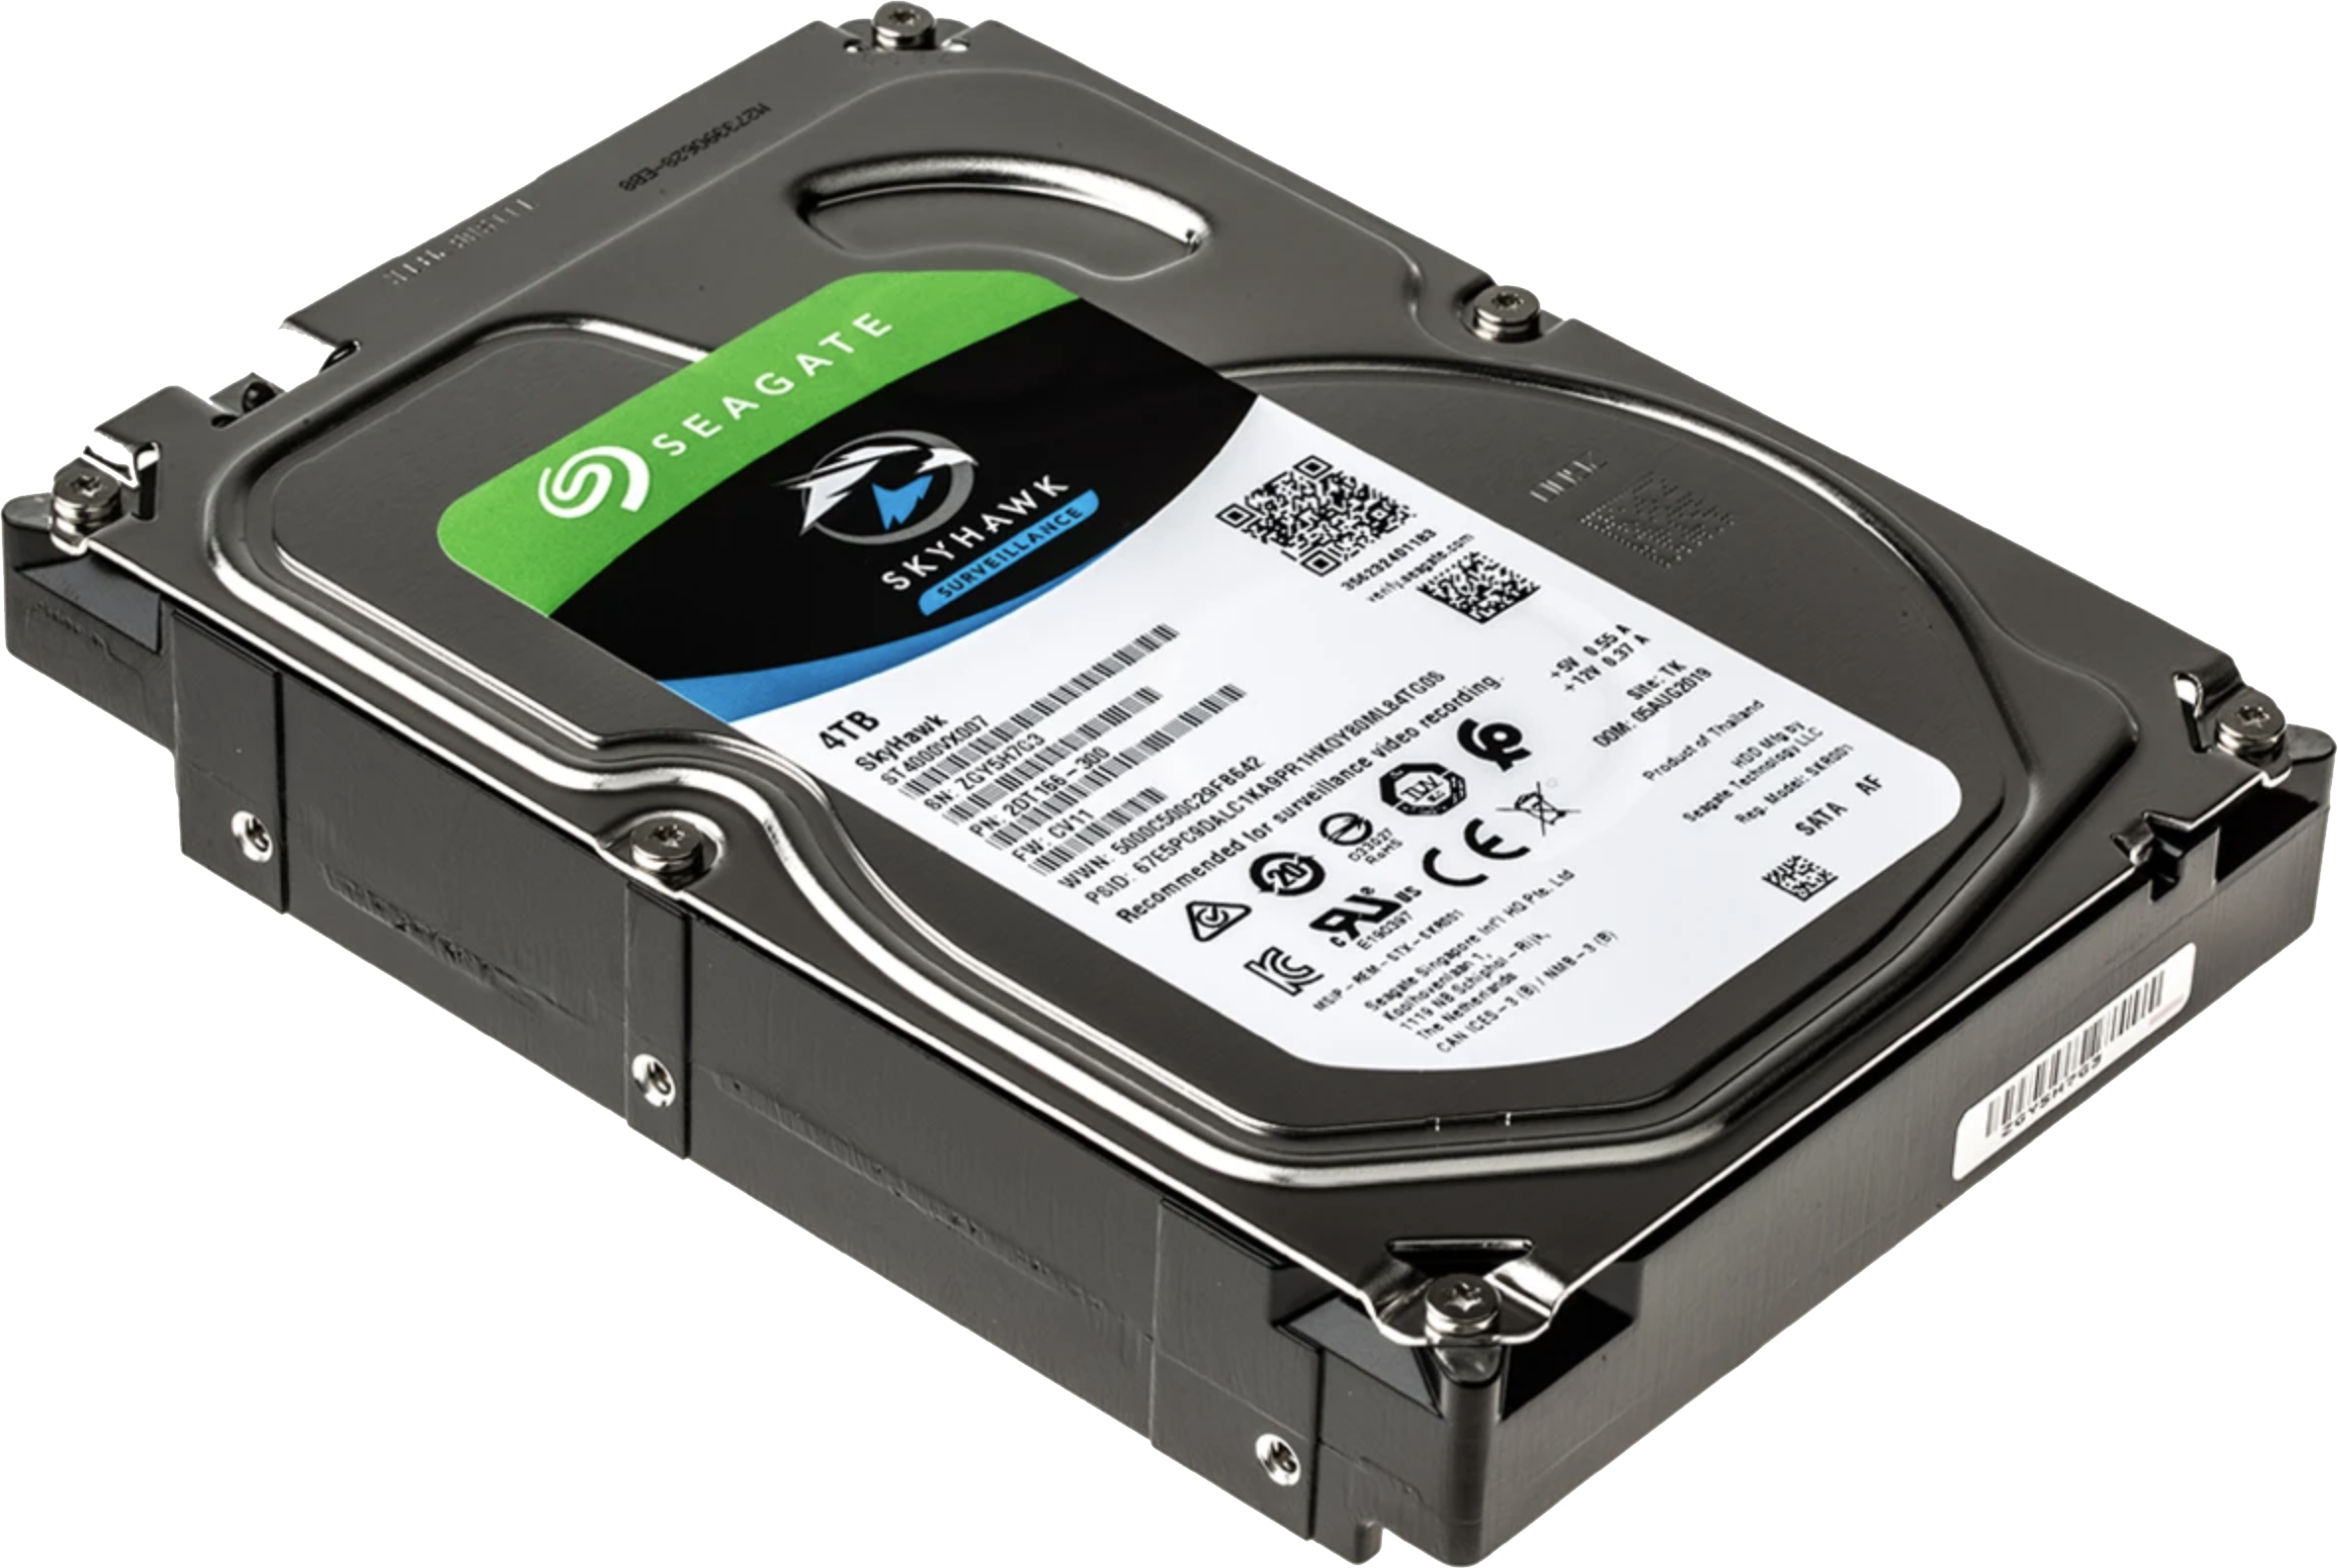
\includegraphics[width=0.6\linewidth]{Figures/harddrive.png}
        \end{wrapfigure}
           Still, although it might not feel so modern, sometimes \alert{if the data
           amount is large} and the \alert{network connections is bad} it might just be
           easiest to transfer the data physically by \alert{shipping a hard drive}.
        \end{block}
    \end{frame}
    \begin{frame}
        \frametitle{Transferring data}
        \framesubtitle{Commercial solution}
        \begin{center}
            Sometimes there might be a commercial solution available
        \end{center}
        \uncover<2->{
        \begin{block}{IBM Aspera}
        \begin{wrapfigure}[4]{r}{0.4\textwidth}
        \vspace{-1.4\baselineskip}
        
\includegraphics[width=0.6\linewidth]{Figures/aspera-logo.png}
        \end{wrapfigure}
            IBM Aspera is a commercial solution for transferring large amount of data.
        \end{block}
        }
    \end{frame}

\subsection{Compression}
    \begin{frame}
        \frametitle{Compression}
        \framesubtitle{zip}
        \begin{block}{zip}
        \begin{wrapfigure}[4]{r}{0.2\textwidth}
        \centering
        \vspace{-6pt}
        
\includegraphics[width=0.55\linewidth]{Figures/zip.png}
        \end{wrapfigure}
            \mbox{}
            \begin{itemize}
                \item Appeared around \alert{1989}
                \item An archive format that \alert{can contain both files and directories} that \alert{can be compressed}
            \end{itemize}
            \mbox{}\vspace{-17pt}
            \begin{itemize}
                \item Built-in zip support in both Windows, Mac OS X and most free operating systems
                \item the name means ``move at high speed''
                \item an index allows for \alert{random access} of files from a zip archive
            \end{itemize}

        \end{block}
    \end{frame}

    \begin{frame}
        \frametitle{Compression}
        \framesubtitle{gz and tar.gz}
        \begin{block}{gzip (gz)}
        \begin{wrapfigure}[4]{r}{0.3\textwidth}
        \centering
        \vspace{-6pt}
        
\includegraphics[width=0.8\linewidth]{Figures/gzip.png}
        \end{wrapfigure}
            \mbox{}

        \begin{itemize}
            \item gzip is a way to compress files
            \item decompression can be done in a streaming fashion
        \end{itemize}
        \end{block}
    \end{frame}

    \begin{frame}
        \frametitle{Compression}
        \framesubtitle{gz and tar.gz}
        \begin{block}{z commands}
            There is a family of special commands to work with gzipped files:
            
            \begin{center}
            \begin{tabular}{rl}
                \texttt{zcat} & View a gzipped file \\
                \texttt{zless} & Browse a gzipped file \\
                \texttt{zgrep} & Search inside a gzipped file \\
                \texttt{zdiff} & Compare gzipped files \\
            \end{tabular}
            \end{center}
        \end{block}
    \end{frame}

\subsection{Storage}
    \begin{frame}
        \frametitle{Databases}
        \framesubtitle{}

        \begin{block}{Databases}
        \small
            You are probably already familiar with \alert{relational databases} (\textit{e.g.}, MySQL) \\[10pt]

            But, with big data \alert{relational databases is not always going to cope}.\\[10pt]


            Although some can spread out over mulitple nodes, \textit{e.g.},
            Postgresql, there are other databases that might be more suited for
            big data, \textit{i.e.}, the \alert{noSQL databases}.
        \end{block}
    \end{frame}
    
    \begin{frame}
        \frametitle{Databases}
        \framesubtitle{NoSQL databases}

        There are databases that don't use SQL and relations. It is good to at
        least have heard about a few of them. Here are a few categories:

        \begin{block}{NoSQL Databases categories}
        \small
        \begin{itemize}
        \item \textbf{Document-oriented}: Stores data as entire documents (\textit{e.g.}, XML, JSON, YAML \ldots)
        \item \textbf{Key-value}: Stores data in associative arrays; what is sometimes
                         called \textit{dictionaries} or \textit{hashes}
        \item \textbf{Graph}: stores graph structures with \textit{nodes} and \textit{edges}
        \end{itemize}
        \end{block}
        There are many more\ldots
    \end{frame}
    
    \begin{frame}
        \frametitle{Databases}
        \framesubtitle{NoSQL databases}
        \begin{block}{Not as complex as relational databases}
            Since the \alert{NoSQL databases} are not as complex as relational
            databases they \alert{can sometimes handle big data much better}, for
            example the document database MongoDB was built to handle really
            large amounts of data.
        \end{block}
    \end{frame}

    \begin{frame}
        \frametitle{Storage when computing}
        \framesubtitle{Local storage / Fast storage}
        \begin{block}{Local storage}
        When working with big data it is important to think about where you
        data is situated. On big computer nodes you can have many different
        kind of storage. Maybe you have large slow storage located far away
        from the compute cores and smaller fast local scratch disks on the
        compute nodes. Depending on the algorithm it \alert{might be well worth
        copying the data to local scratch disks} first.
        \end{block}
    \end{frame}

\section{Apache Spark}
\begin{frame}[plain]
\hfill\LARGE Apache Spark \hfill\normalsize
\end{frame}
    \subsection{Background}
\setbeamertemplate{background}{%
    \parbox[c][\paperheight]{\paperwidth}{%
        \vskip -0.1 ex \hskip -1 em
        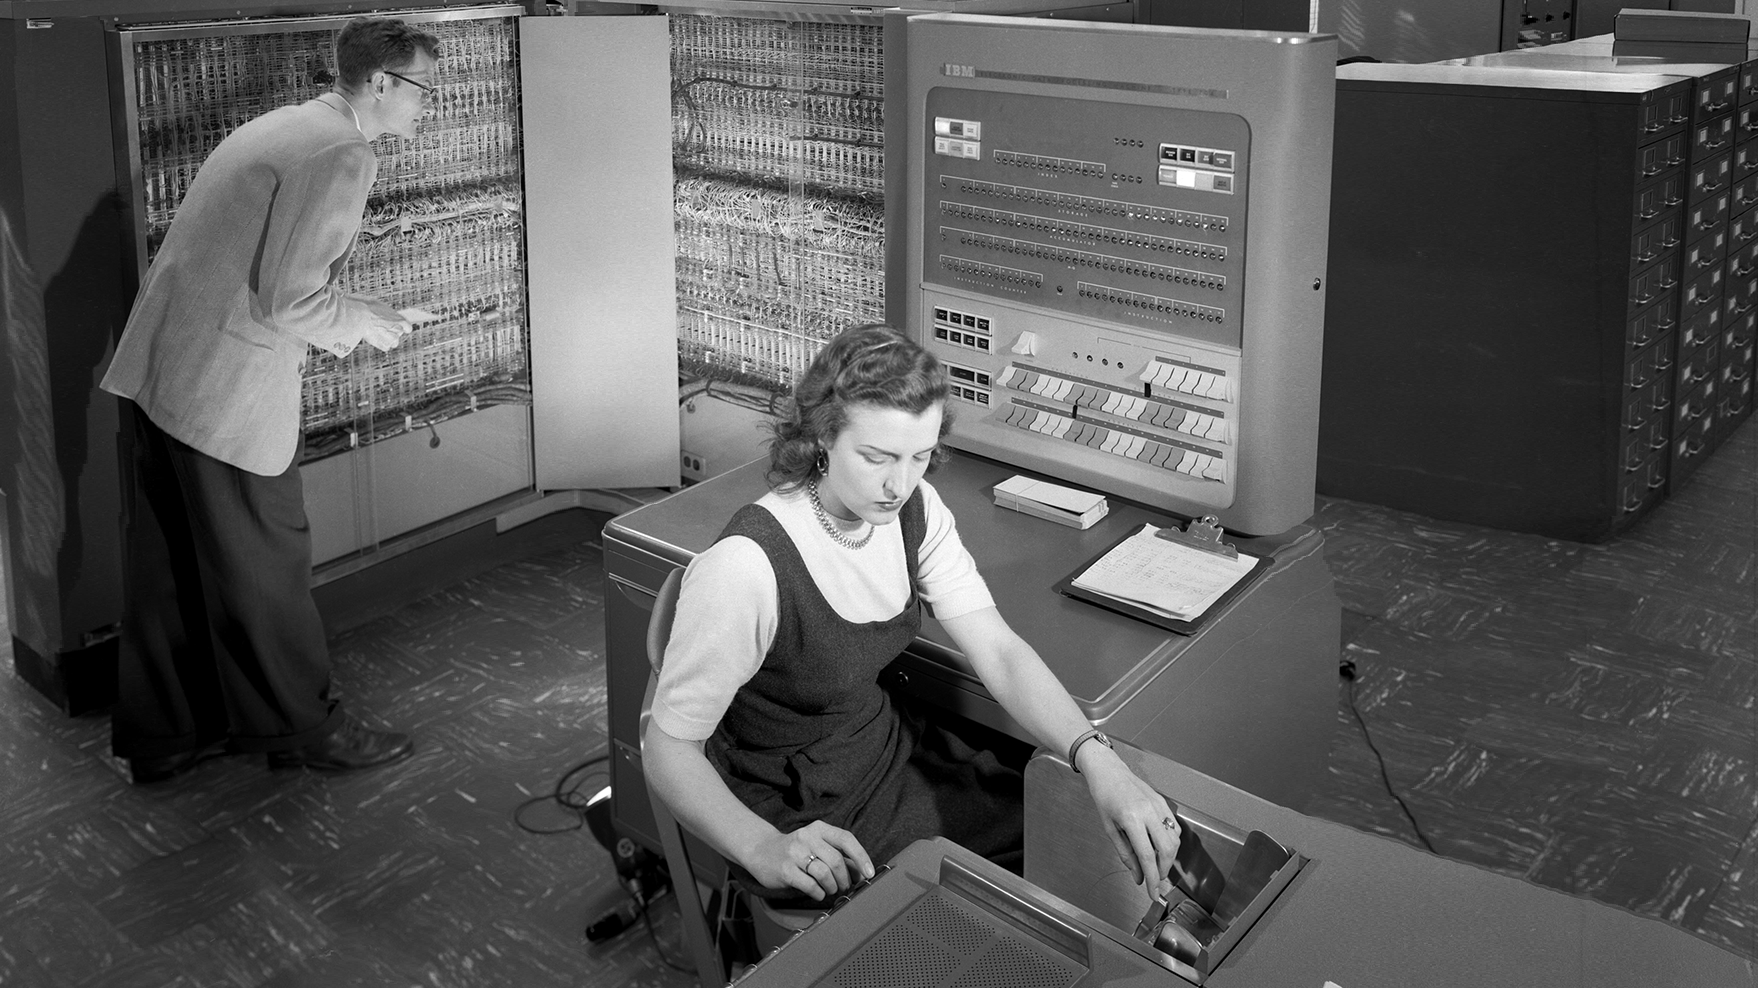
\includegraphics[width=1.05\paperwidth]{Figures/LISP.png}
    }   
}
\begin{frame}[plain]
        %\vskip -20 ex
    %\Large\qquad\qquad\qquad\color{black} {\zA In the beginning there was} \\
    %\Huge LISP
\hfill        {\small\color{white}IBM 704 Computer in 1957}
\vfill\vfill\vfill\vfill\vfill
\begin{minipage}[c]{0.5\textwidth}
        \pause
        \oldBlock{\zA "In the beginning there was":}
        \begin{center}
        \vspace*{2ex}
        \Huge LISP
        \vspace*{1ex}
        \end{center}
        \endoldBlock
\end{minipage}\hfill


\end{frame}
\setbeamertemplate{background}{}
    \begin{frame}
        \frametitle{LISP}
        \framesubtitle{LISt Processor}
            \begin{center}\texttt{(print "Hello, World!")}\end{center}
        \begin{block}{LISP}
            \begin{itemize}
                \item created in 1958
                \item is the second-oldest high-level programming language in widespread use today (the oldest being FORTRAN)
            \end{itemize}
        \end{block}

    \end{frame}
    \begin{frame}[fragile]
        \frametitle{LISP}
        \framesubtitle{LISt Processor}
\begin{minipage}{0.42\textwidth}
\raggedright
LISP is a powerful, but in my opinion, somewhat special language. Here is an example\footnotemark calculating the factorial of a number {\small (directly from Wikipedia)}:
\begin{lstlisting}
(defun factorial (n)
    (if (= n 0) 1
        (* n (factorial (- n 1)))))
\end{lstlisting}
\end{minipage}
\hfill
\uncover<2->{
\begin{minipage}{0.55\textwidth}
\centering
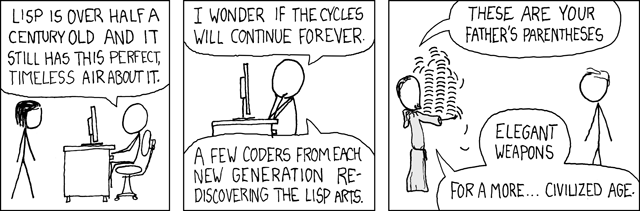
\includegraphics[width=1\textwidth]{Figures/lisp_cycles.png}
\small \texttt{https://xkcd.com/297/}
\end{minipage}}
\footnotetext{You do \alert{\underline{not}} need to learn LISP in this course}
    \end{frame}

    \begin{frame}
        \frametitle{Map and Reduce}
        \color{lightgray}
        \begin{center}
            \only<1->{\only<1>{\color{black}}So, why do I talk so much about LISP?}
        \end{center}
        \begin{center}
            \only<2->{\only<2>{\color{black}}It's because its list-based structure lent itself well for \texttt{map} and \texttt{reduce}}
        \end{center}
        \begin{center}
            \only<3->{\only<3>{\color{black}}Which later gave rise to the MapReduce programming model}
        \end{center}
        \begin{center}
            \only<4->{\only<4>{\color{black}}but first, let's talk about \texttt{map} and \texttt{reduce}\ldots}
        \end{center}
    \end{frame}

    \begin{frame}[fragile]
        \frametitle{Map and Reduce}
        \framesubtitle{Map}

            \begin{block}{Map}
                \texttt{map} is a higher-order function that applies a given
                function to each element of, \textit{e.g.}, a list. It can also
                be called \texttt{apply-to-all}.
            \end{block}
            \begin{uncoverenv}<2->
            \begin{block}{Example: \hfill \small(Python)}
            \begin{center}
            \begin{minipage}{0.8\linewidth}
            \begin{lstlisting}
square = lambda x:x*x
a = [1,2,3,4]
list(map(square, a))
            \end{lstlisting}
            $\Rightarrow$ \texttt{[1, 4, 9, 16]}
            \end{minipage}
            \end{center}
            \end{block}
            \end{uncoverenv}
        
    \end{frame}
    
    \begin{frame}[fragile]
        \frametitle{Map and Reduce}
        \framesubtitle{Reduce}

            \begin{block}{Reduce}
                \texttt{reduce} is a higher-order function that by using a
                given function combines the part of, \textit{e.g.}, a list into
                a return value.
            \end{block}
            \begin{uncoverenv}<2->
            \begin{block}{Example: \hfill \small(Python)}
            \begin{center}
            \begin{minipage}{0.8\linewidth}
            \begin{lstlisting}
from functools import reduce
sum = lambda a,b:a+b
a = [1,2,3,4]
reduce(sum,a)
            \end{lstlisting}
            $\Rightarrow$ 10
            \end{minipage}
            \end{center}
            \end{block}
            \end{uncoverenv}
    \end{frame}

    \begin{frame}
        \frametitle{Map and Reduce}
        \framesubtitle{Map and Reduce}

        \vspace{-4ex}
        \begin{block}{Map and Reduce}
    \centering
    \begin{tikzpicture}[node distance=0]
      \only<1>{
        \node (a)  [draw,circle, minimum size=8pt]{};
        \node (b)  [right of = a, node distance = 16 pt, draw,circle, minimum size=8pt]{};
        \node (c)  [right of = b, node distance = 16 pt, draw,circle, minimum size=8pt]{};
        \node (d)  [right of = c, node distance = 16 pt, draw,circle, minimum size=8pt]{};
        \node (e)  [right of = d, node distance = 16 pt, draw,circle, minimum size=8pt]{};
        \node (f)  [right of = e, node distance = 16 pt, draw,circle, minimum size=8pt]{};
        \node (g)  [right of = f, node distance = 16 pt, draw,circle, minimum size=8pt]{};
        \node (h)  [right of = g, node distance = 16 pt, draw,circle, minimum size=8pt]{};
        \node (i)  [right of = h, node distance = 16 pt, draw,circle, minimum size=8pt]{};
        \node (j)  [right of = i, node distance = 16 pt, draw,circle, minimum size=8pt]{};
        
        \node (aa)  [below of = a, node distance = 32 pt, draw,circle, minimum size=8pt]{};
        \node (ab)  [right of = aa, node distance = 16 pt, draw,circle, minimum size=8pt]{};
        \node (ac)  [right of = ab, node distance = 16 pt, draw,circle, minimum size=8pt]{};
        \node (ad)  [right of = ac, node distance = 16 pt, draw,circle, minimum size=8pt]{};
        \node (ae)  [right of = ad, node distance = 16 pt, draw,circle, minimum size=8pt]{};
        \node (af)  [right of = ae, node distance = 16 pt, draw,circle, minimum size=8pt]{};
        \node (ag)  [right of = af, node distance = 16 pt, draw,circle, minimum size=8pt]{};
        \node (ah)  [right of = ag, node distance = 16 pt, draw,circle, minimum size=8pt]{};
        \node (ai)  [right of = ah, node distance = 16 pt, draw,circle, minimum size=8pt]{};
        \node (aj)  [right of = ai, node distance = 16 pt, draw,circle, minimum size=8pt]{};

        \draw [->, shorten <=3pt, shorten >=3pt] (a) to (aa);
        \draw [->, shorten <=3pt, shorten >=3pt] (b) to (ab);
        \draw [->, shorten <=3pt, shorten >=3pt] (c) to (ac);
        \draw [->, shorten <=3pt, shorten >=3pt] (d) to (ad);
        \draw [->, shorten <=3pt, shorten >=3pt] (e) to (ae);
        \draw [->, shorten <=3pt, shorten >=3pt] (f) to (af);
        \draw [->, shorten <=3pt, shorten >=3pt] (g) to (ag);
        \draw [->, shorten <=3pt, shorten >=3pt] (h) to (ah);
        \draw [->, shorten <=3pt, shorten >=3pt] (i) to (ai);
        \draw [->, shorten <=3pt, shorten >=3pt] (j) to (aj);

        \node (startbrace1) [node distance = 10 pt, above right of = j] {};
        \node (stopbrace1) [node distance = 10 pt, below right of = aj, yshift=4pt] {};
        \draw [decorate,decoration={brace,amplitude=10pt,raise=4pt}]
              (startbrace1) -- (stopbrace1) node [black,midway,xshift=1.05cm] {Map};
      }
      \uncover<3->{
        \node (a)  [draw,circle, minimum size=8pt]{};
        \node (b)  [right of = a, node distance = 16 pt, draw,circle, minimum size=8pt]{};
        \node (c)  [right of = b, node distance = 16 pt, draw,circle, minimum size=8pt]{};
        \node (d)  [right of = c, node distance = 16 pt, draw,circle, minimum size=8pt]{};
        \node (e)  [right of = d, node distance = 16 pt, draw,circle, minimum size=8pt]{};
        \node (f)  [right of = e, node distance = 16 pt, draw,circle, minimum size=8pt]{};
        \node (g)  [right of = f, node distance = 16 pt, draw,circle, minimum size=8pt]{};
        \node (h)  [right of = g, node distance = 16 pt, draw,circle, minimum size=8pt]{};
        \node (i)  [right of = h, node distance = 16 pt, draw,circle, minimum size=8pt]{};
        \node (j)  [right of = i, node distance = 16 pt, draw,circle, minimum size=8pt]{};
      }
       
      \only<2>{
        \node (aa)  [below of = a, node distance = 32 pt, draw,circle, minimum size=8pt]{};
        \node (ab)  [right of = aa, node distance = 16 pt, draw,circle, minimum size=8pt]{};
        \node (ac)  [right of = ab, node distance = 16 pt, draw,circle, minimum size=8pt]{};
        \node (ad)  [right of = ac, node distance = 16 pt, draw,circle, minimum size=8pt]{};
        \node (ae)  [right of = ad, node distance = 16 pt, draw,circle, minimum size=8pt]{};
        \node (af)  [right of = ae, node distance = 16 pt, draw,circle, minimum size=8pt]{};
        \node (ag)  [right of = af, node distance = 16 pt, draw,circle, minimum size=8pt]{};
        \node (ah)  [right of = ag, node distance = 16 pt, draw,circle, minimum size=8pt]{};
        \node (ai)  [right of = ah, node distance = 16 pt, draw,circle, minimum size=8pt]{};
        \node (aj)  [right of = ai, node distance = 16 pt, draw,circle, minimum size=8pt]{};
      }
      \uncover<3->{
        \draw [->, shorten <=3pt, shorten >=3pt] (a) to (aa);
        \draw [->, shorten <=3pt, shorten >=3pt] (b) to (ab);
        \draw [->, shorten <=3pt, shorten >=3pt] (c) to (ac);
        \draw [->, shorten <=3pt, shorten >=3pt] (d) to (ad);
        \draw [->, shorten <=3pt, shorten >=3pt] (e) to (ae);
        \draw [->, shorten <=3pt, shorten >=3pt] (f) to (af);
        \draw [->, shorten <=3pt, shorten >=3pt] (g) to (ag);
        \draw [->, shorten <=3pt, shorten >=3pt] (h) to (ah);
        \draw [->, shorten <=3pt, shorten >=3pt] (i) to (ai);
        \draw [->, shorten <=3pt, shorten >=3pt] (j) to (aj);
      }

      \only<2>{
        \node (startbrace1) [node distance = 10 pt, above right of = j] {};
        \node (stopbrace1) [node distance = 10 pt, below right of = aj, yshift=4pt] {};
        
        \node (ba)  [below of = aa, node distance = 24 pt, xshift=8pt, draw, circle, minimum size=8pt]{};
        \node (bb)  [below of = ac, node distance = 24 pt, xshift=8pt, draw, circle, minimum size=8pt]{};
        \node (bc)  [below of = ae, node distance = 24 pt, xshift=8pt, draw, circle, minimum size=8pt]{};
        \node (bd)  [below of = ag, node distance = 24 pt, xshift=8pt, draw, circle, minimum size=8pt]{};
        \node (be)  [below of = ai, node distance = 24 pt, xshift=8pt, draw, circle, minimum size=8pt]{};
        
        \node (ca)  [below of = ba, node distance = 24 pt, xshift=16pt, draw, circle, minimum size=8pt]{};
        \node (cb)  [below of = bc, node distance = 24 pt, xshift=16pt, draw, circle, minimum size=8pt]{};
        
        \node (da)  [below of = ca, node distance = 36 pt, xshift=48pt, draw, circle, minimum size=8pt]{};
        \node (db)  [below of = bd, node distance = 36 pt, xshift=16pt, draw, circle, minimum size=8pt]{};
        
        \draw [->, shorten <=3pt, shorten >=3pt] (aa) to (ba);
        \draw [->, shorten <=3pt, shorten >=3pt] (ab) to (ba);
        \draw [->, shorten <=3pt, shorten >=3pt] (ac) to (bb);
        \draw [->, shorten <=3pt, shorten >=3pt] (ad) to (bb);
        \draw [->, shorten <=3pt, shorten >=3pt] (ae) to (bc);
        \draw [->, shorten <=3pt, shorten >=3pt] (af) to (bc);
        \draw [->, shorten <=3pt, shorten >=3pt] (ag) to (bd);
        \draw [->, shorten <=3pt, shorten >=3pt] (ah) to (bd);
        \draw [->, shorten <=3pt, shorten >=3pt] (ai) to (be);
        \draw [->, shorten <=3pt, shorten >=3pt] (aj) to (be);
        
        \draw [->, shorten <=3pt, shorten >=3pt] (ba) to (ca);
        \draw [->, shorten <=3pt, shorten >=3pt] (bb) to (ca);
        \draw [->, shorten <=3pt, shorten >=3pt] (bc) to (cb);
        \draw [->, shorten <=3pt, shorten >=3pt] (bd) to (cb);
        
        \draw [->, shorten <=3pt, shorten >=3pt] (cb) to (db);
        \draw [->, shorten <=3pt, shorten >=3pt] (be) to (db);
        
        \draw [->, shorten <=3pt, shorten >=3pt] (ca) to (da);
        \draw [->, shorten <=3pt, shorten >=3pt] (db) to (da);
        
        
        \node (startbrace2) [node distance = 10 pt, below right of = aj, yshift=10pt] {};
        \node (stopbrace2) [node distance = 3.4 cm, below of = startbrace2] {};

        \draw [decorate,decoration={brace,amplitude=10pt,raise=4pt}]
              (startbrace2) -- (stopbrace2) node [black,midway,xshift=1.17cm] {Reduce};
      }
      \only<3->{
        \node (aa)  [below of = a, node distance = 32 pt, draw,circle, minimum size=8pt]{};
        \node (ab)  [right of = aa, node distance = 16 pt, draw,circle, minimum size=8pt]{};
        \node (ac)  [right of = ab, node distance = 16 pt, draw,circle, minimum size=8pt]{};
        \node (ad)  [right of = ac, node distance = 16 pt, draw,circle, minimum size=8pt]{};
        \node (ae)  [right of = ad, node distance = 16 pt, draw,circle, minimum size=8pt]{};
        \node (af)  [right of = ae, node distance = 16 pt, draw,circle, minimum size=8pt]{};
        \node (ag)  [right of = af, node distance = 16 pt, draw,circle, minimum size=8pt]{};
        \node (ah)  [right of = ag, node distance = 16 pt, draw,circle, minimum size=8pt]{};
        \node (ai)  [right of = ah, node distance = 16 pt, draw,circle, minimum size=8pt]{};
        \node (aj)  [right of = ai, node distance = 16 pt, draw,circle, minimum size=8pt]{};
      }
      \only<3->{
        \node (ba)  [below of = aa, node distance = 24 pt, xshift=8pt, draw, circle, minimum size=8pt]{};
        \node (bb)  [below of = ac, node distance = 24 pt, xshift=8pt, draw, circle, minimum size=8pt]{};
        \node (bc)  [below of = ae, node distance = 24 pt, xshift=8pt, draw, circle, minimum size=8pt]{};
        \node (bd)  [below of = ag, node distance = 24 pt, xshift=8pt, draw, circle, minimum size=8pt]{};
        \node (be)  [below of = ai, node distance = 24 pt, xshift=8pt, draw, circle, minimum size=8pt]{};
        
        \node (ca)  [below of = ba, node distance = 24 pt, xshift=16pt, draw, circle, minimum size=8pt]{};
        \node (cb)  [below of = bc, node distance = 24 pt, xshift=16pt, draw, circle, minimum size=8pt]{};
        
        \node (da)  [below of = ca, node distance = 36 pt, xshift=48pt, draw, circle, minimum size=8pt]{};
        \node (db)  [below of = bd, node distance = 36 pt, xshift=16pt, draw, circle, minimum size=8pt]{};
        
        \draw [->, shorten <=3pt, shorten >=3pt] (aa) to (ba);
        \draw [->, shorten <=3pt, shorten >=3pt] (ab) to (ba);
        \draw [->, shorten <=3pt, shorten >=3pt] (ac) to (bb);
        \draw [->, shorten <=3pt, shorten >=3pt] (ad) to (bb);
        \draw [->, shorten <=3pt, shorten >=3pt] (ae) to (bc);
        \draw [->, shorten <=3pt, shorten >=3pt] (af) to (bc);
        \draw [->, shorten <=3pt, shorten >=3pt] (ag) to (bd);
        \draw [->, shorten <=3pt, shorten >=3pt] (ah) to (bd);
        \draw [->, shorten <=3pt, shorten >=3pt] (ai) to (be);
        \draw [->, shorten <=3pt, shorten >=3pt] (aj) to (be);
        
        \draw [->, shorten <=3pt, shorten >=3pt] (ba) to (ca);
        \draw [->, shorten <=3pt, shorten >=3pt] (bb) to (ca);
        \draw [->, shorten <=3pt, shorten >=3pt] (bc) to (cb);
        \draw [->, shorten <=3pt, shorten >=3pt] (bd) to (cb);
        
        \draw [->, shorten <=3pt, shorten >=3pt] (cb) to (db);
        \draw [->, shorten <=3pt, shorten >=3pt] (be) to (db);
        
        \draw [->, shorten <=3pt, shorten >=3pt] (ca) to (da);
        \draw [->, shorten <=3pt, shorten >=3pt] (db) to (da);
      } 
      \only<1>{ 
        \node (startbrace2) [node distance = 10 pt, below right of = aj, yshift=10pt] {};
        \node (stopbrace2) [node distance = 3.4 cm, below of = startbrace2] {};
      }
      \uncover<3->{
        \draw [decorate,decoration={brace,amplitude=10pt,raise=4pt}]
              (startbrace1) -- (stopbrace2) node (mapreduce) [black,midway,xshift=2.7cm] {Map followed by reduce};

      }
      \uncover<4>{
            \node [node distance = 36 pt, below of = mapreduce] {
                \begin{minipage}{0.3\textwidth}
                    \textcolor{darkpastelgreen}{(Of course you don't \textit{have to} finish with reduce)}
                \end{minipage}
                };
      }
    \end{tikzpicture}
        
    \end{block}
    \end{frame}

    \begin{frame}
        \frametitle{Map and Reduce}
        \framesubtitle{Map and Reduce}
        \begin{block}{Learning to work with map and reduce}
            \begin{itemize}
                \item Map and reduce can be used with \alert{many languages} so it is a \alert{general skill} worth learning
                \item Just make sure that you \alert{know what you have in your list!}
            \end{itemize}
        \end{block}
    \end{frame}

    \begin{frame}
        \frametitle{MapReduce frameworks}
        \framesubtitle{Parallelisation}
        \begin{block}{MapReduce frameworks are parallel}
        Since each step in Map and Reduce is separate it lends itself well to
        parallelisation. The idea behind \alert{MapReduce} frameworks is to run in
        \alert{massively parallel} ways.
        \end{block}
    \end{frame}


{
    \setbeamercolor{background canvas}{bg=black}
    \setbeamercolor{normal text}{fg=white}\usebeamercolor*{normal text}
    \setbeamercolor{item}{fg=white, bg=black}
    
    \begin{frame}[plain]
        \begin{center}
        Let's take a step back,
        \end{center}
    \end{frame}
    
    \setbeamertemplate{background}{%
    \parbox[c][\paperheight]{\paperwidth}{%
        \vskip -0.1 ex \hskip -1 em
        
\includegraphics[width=1.05\paperwidth]{Figures/question-mark.jpg}
    }   
    }

    \begin{frame}[plain]
        \begin{center}
            \vspace{0.65\textheight}
            \Huge \textbf{Why are we doing this?}
        \end{center}
    \end{frame}
    \setbeamertemplate{background}{%
        \parbox[c][\paperheight]{\paperwidth}{%
            \vskip -0.1 ex \hskip -1 em
            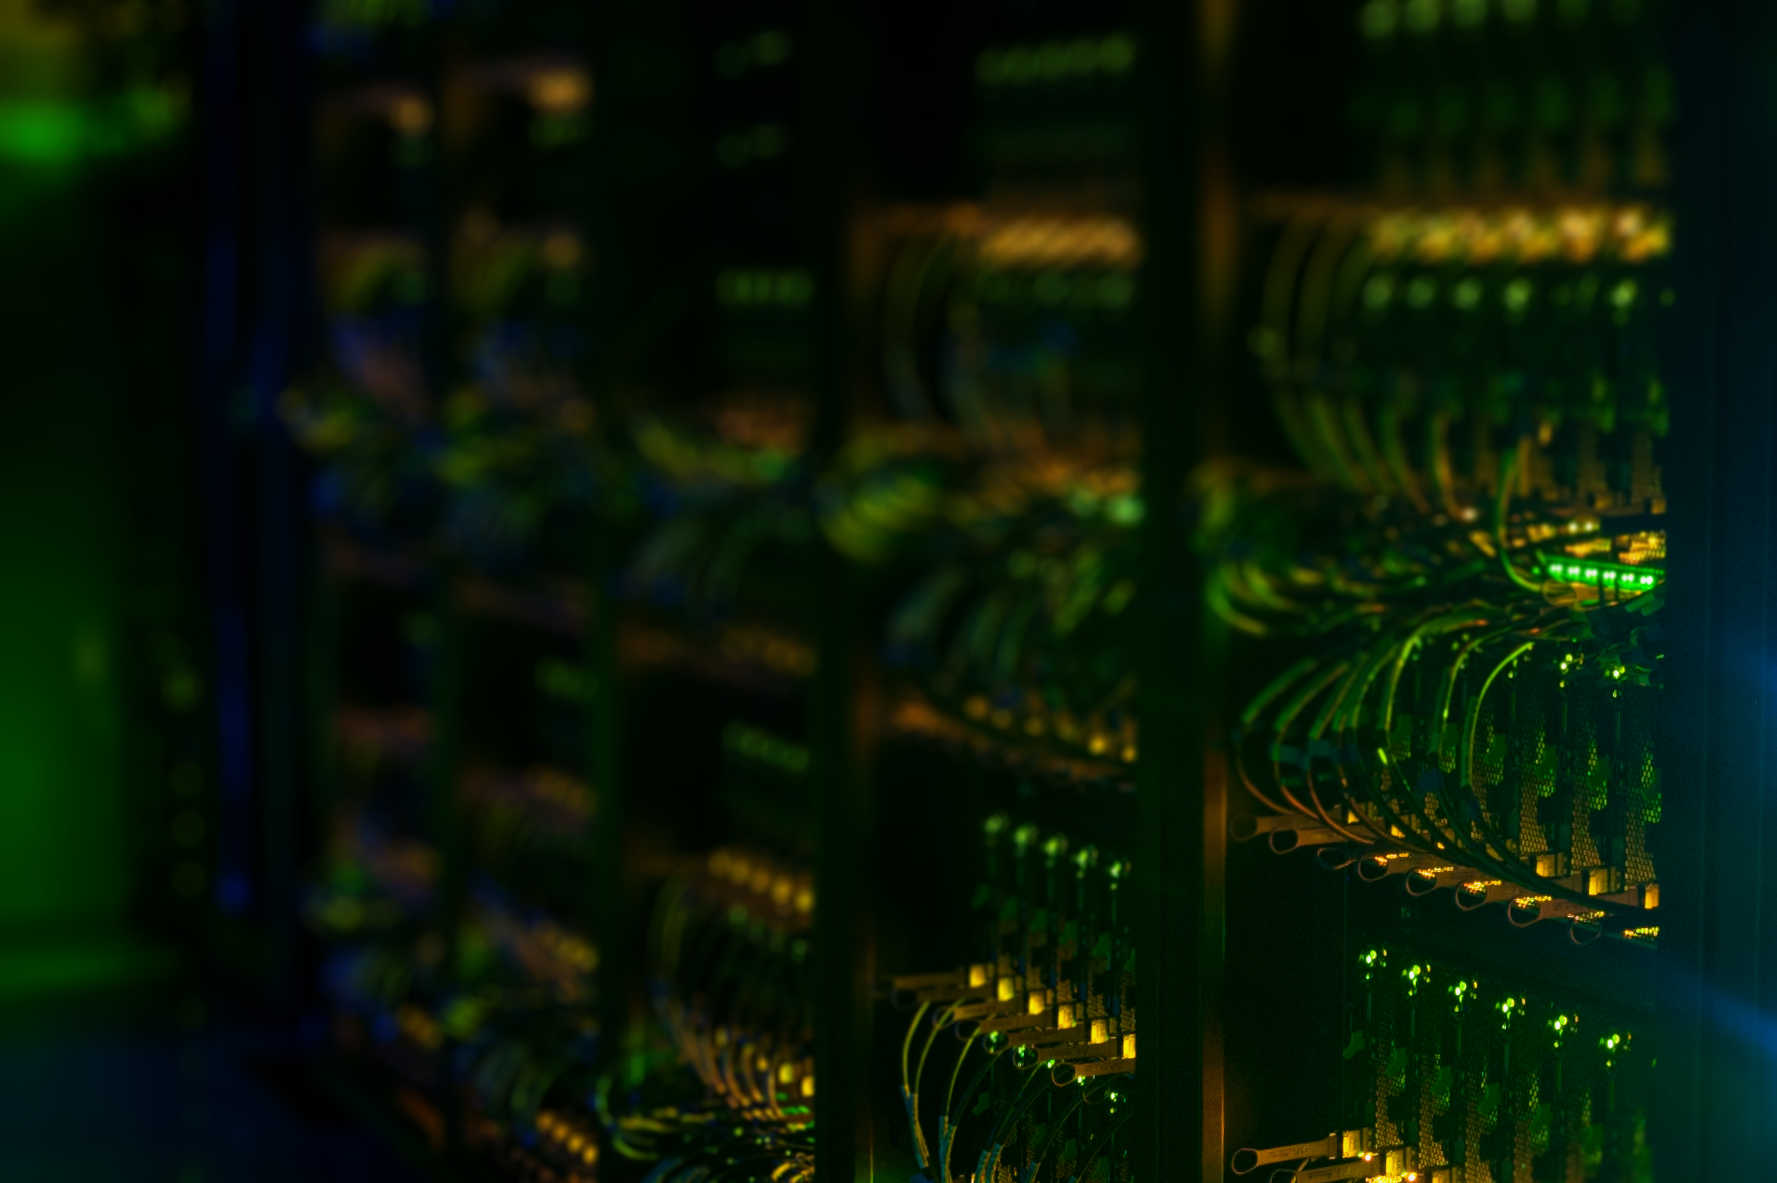
\includegraphics[width=1.05\paperwidth]{Figures/uppmax.png}
        } 
    }
    \begin{frame}[plain]
        \begin{center}
            \Huge Parallel computing! \pause
            \vspace{0.15\textheight}

            \Large These days even the new iPhones have a bunch of cores\ldots 
            
            \vspace{0.05\textheight}

            \normalsize and when you have a big data you want to\pause
            
            \vspace{0.1\textheight}
            
            \Huge run in parallel!
        \end{center}
    \end{frame}
}
       
    \begin{frame}
        \frametitle{MapReduce frameworks}
        \framesubtitle{Parallelisation}
        \begin{block}{Apache Hadoop}
        \begin{wrapfigure}[2]{r}{0.45\textwidth}
        \vspace{-1.2\baselineskip}
        
\includegraphics[width=1\linewidth]{figures/hadoop.png}
        \end{wrapfigure}
        Apache Hadoop is an example of a MapReduce framework that:
        \begin{itemize}
            \item Was \alert{released in 2006}
            \item Works by loading things \alert{from disk}, performing map and reduce operations and then \alert{writing back to disk}.
            \item Can use relatively \alert{cheap computers} to run things in \alert{parallel}
            \item Has relatively \alert{hard APIs to code against} while doing the map and reduce operations
        \end{itemize}
        \end{block}
    \end{frame}

    \begin{frame}
        \frametitle{MapReduce frameworks}
        \framesubtitle{Parallelisation}
        \centering
        In the Spark laboration we will load a file from the Hadoop file system:
        \begin{block}{Hadoop File System (HDFS)}
            The Hadoop File system (HDFS) is a \alert{distributed},
            \alert{scalable} storage solution designed for large data.
        \end{block}
    \end{frame}
    


\subsection{Spark}
    \begin{frame}
        \frametitle{Spark}
        \framesubtitle{``a unified analytics engine for large-scale data processing''}
        \vspace{-3ex}
        \begin{block}{Apache Spark}
        \begin{wrapfigure}[3]{r}{0.35\textwidth}
        \vspace{-1\baselineskip}
        
\includegraphics[width=0.9\linewidth]{figures/Spark.png}\hfill
        \end{wrapfigure}
        In \alert{2014} Spark was released, in a way as a sort of response to Hadoop. Spark:
        \begin{itemize}
            \item Keeps things \alert{in memory} and is thus faster than Hadoop
        \end{itemize}\vspace{-4pt}

        \begin{itemize}
            \item Has \alert{friendly API}s for Python, Scala and to some degree R
            \item Has \alert{better support for machine learning} than Hadoop
            \item Requires \alert{relatively expensive computers} to run because it
            needs huge amounts of RAM if it is to benefit from keeping all data
            in memory.
        \end{itemize}
        \end{block}
    \end{frame}

    \begin{frame}
        \frametitle{Spark}
        \framesubtitle{``a unified analytics engine for large-scale data processing''}
        \vspace{-3ex}
        \begin{block}{Apache Spark}
        \begin{center}
            \only<1>{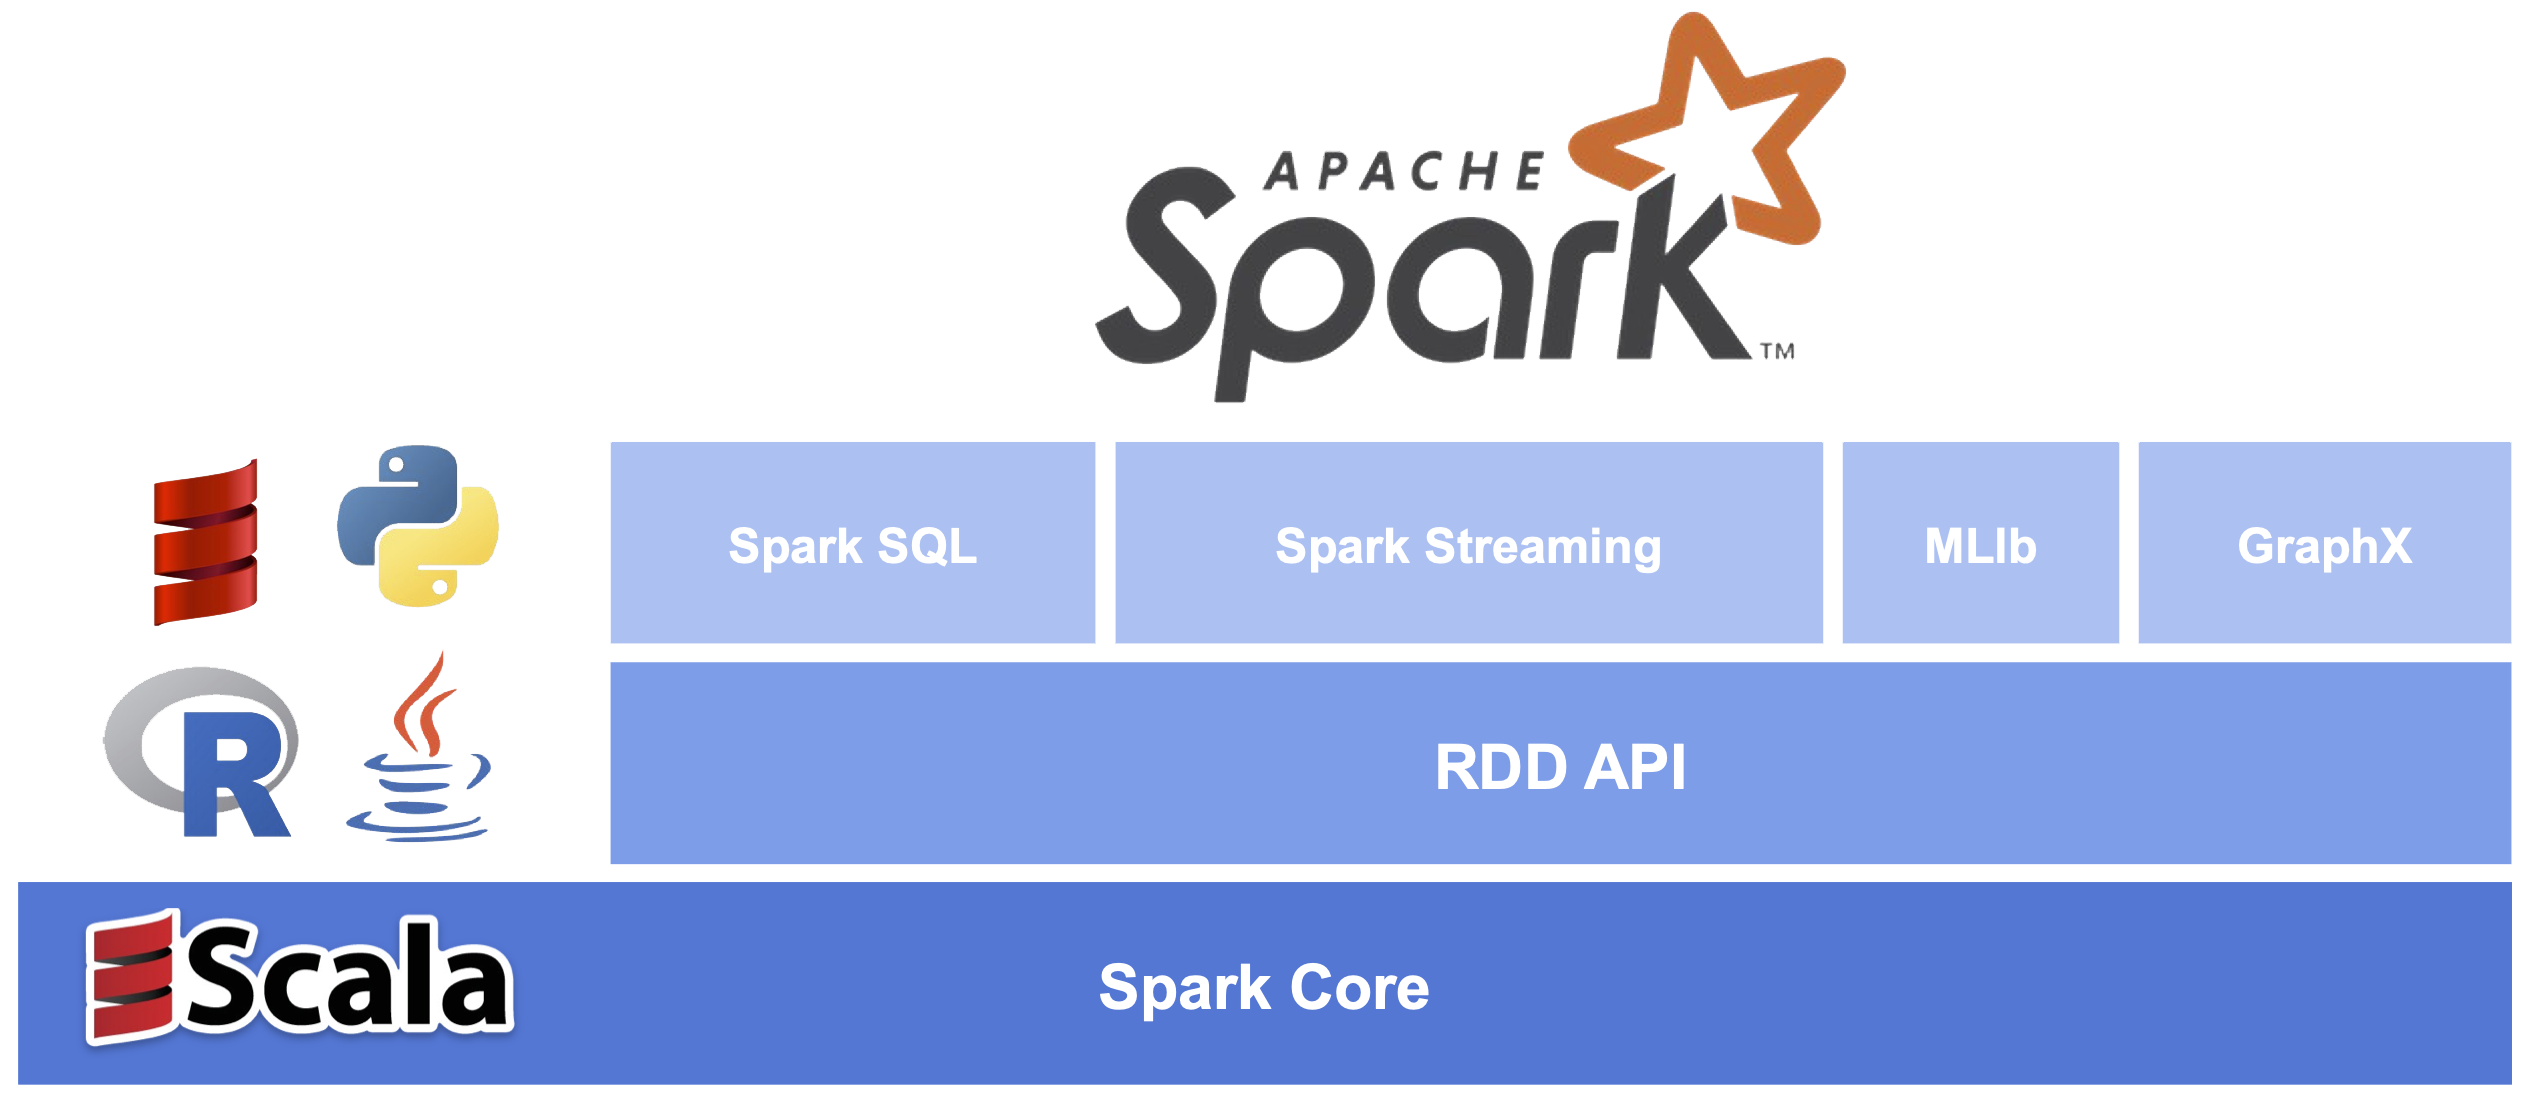
\includegraphics[width=0.9\textwidth]{figures/spark-overview.png}}
            \only<2>{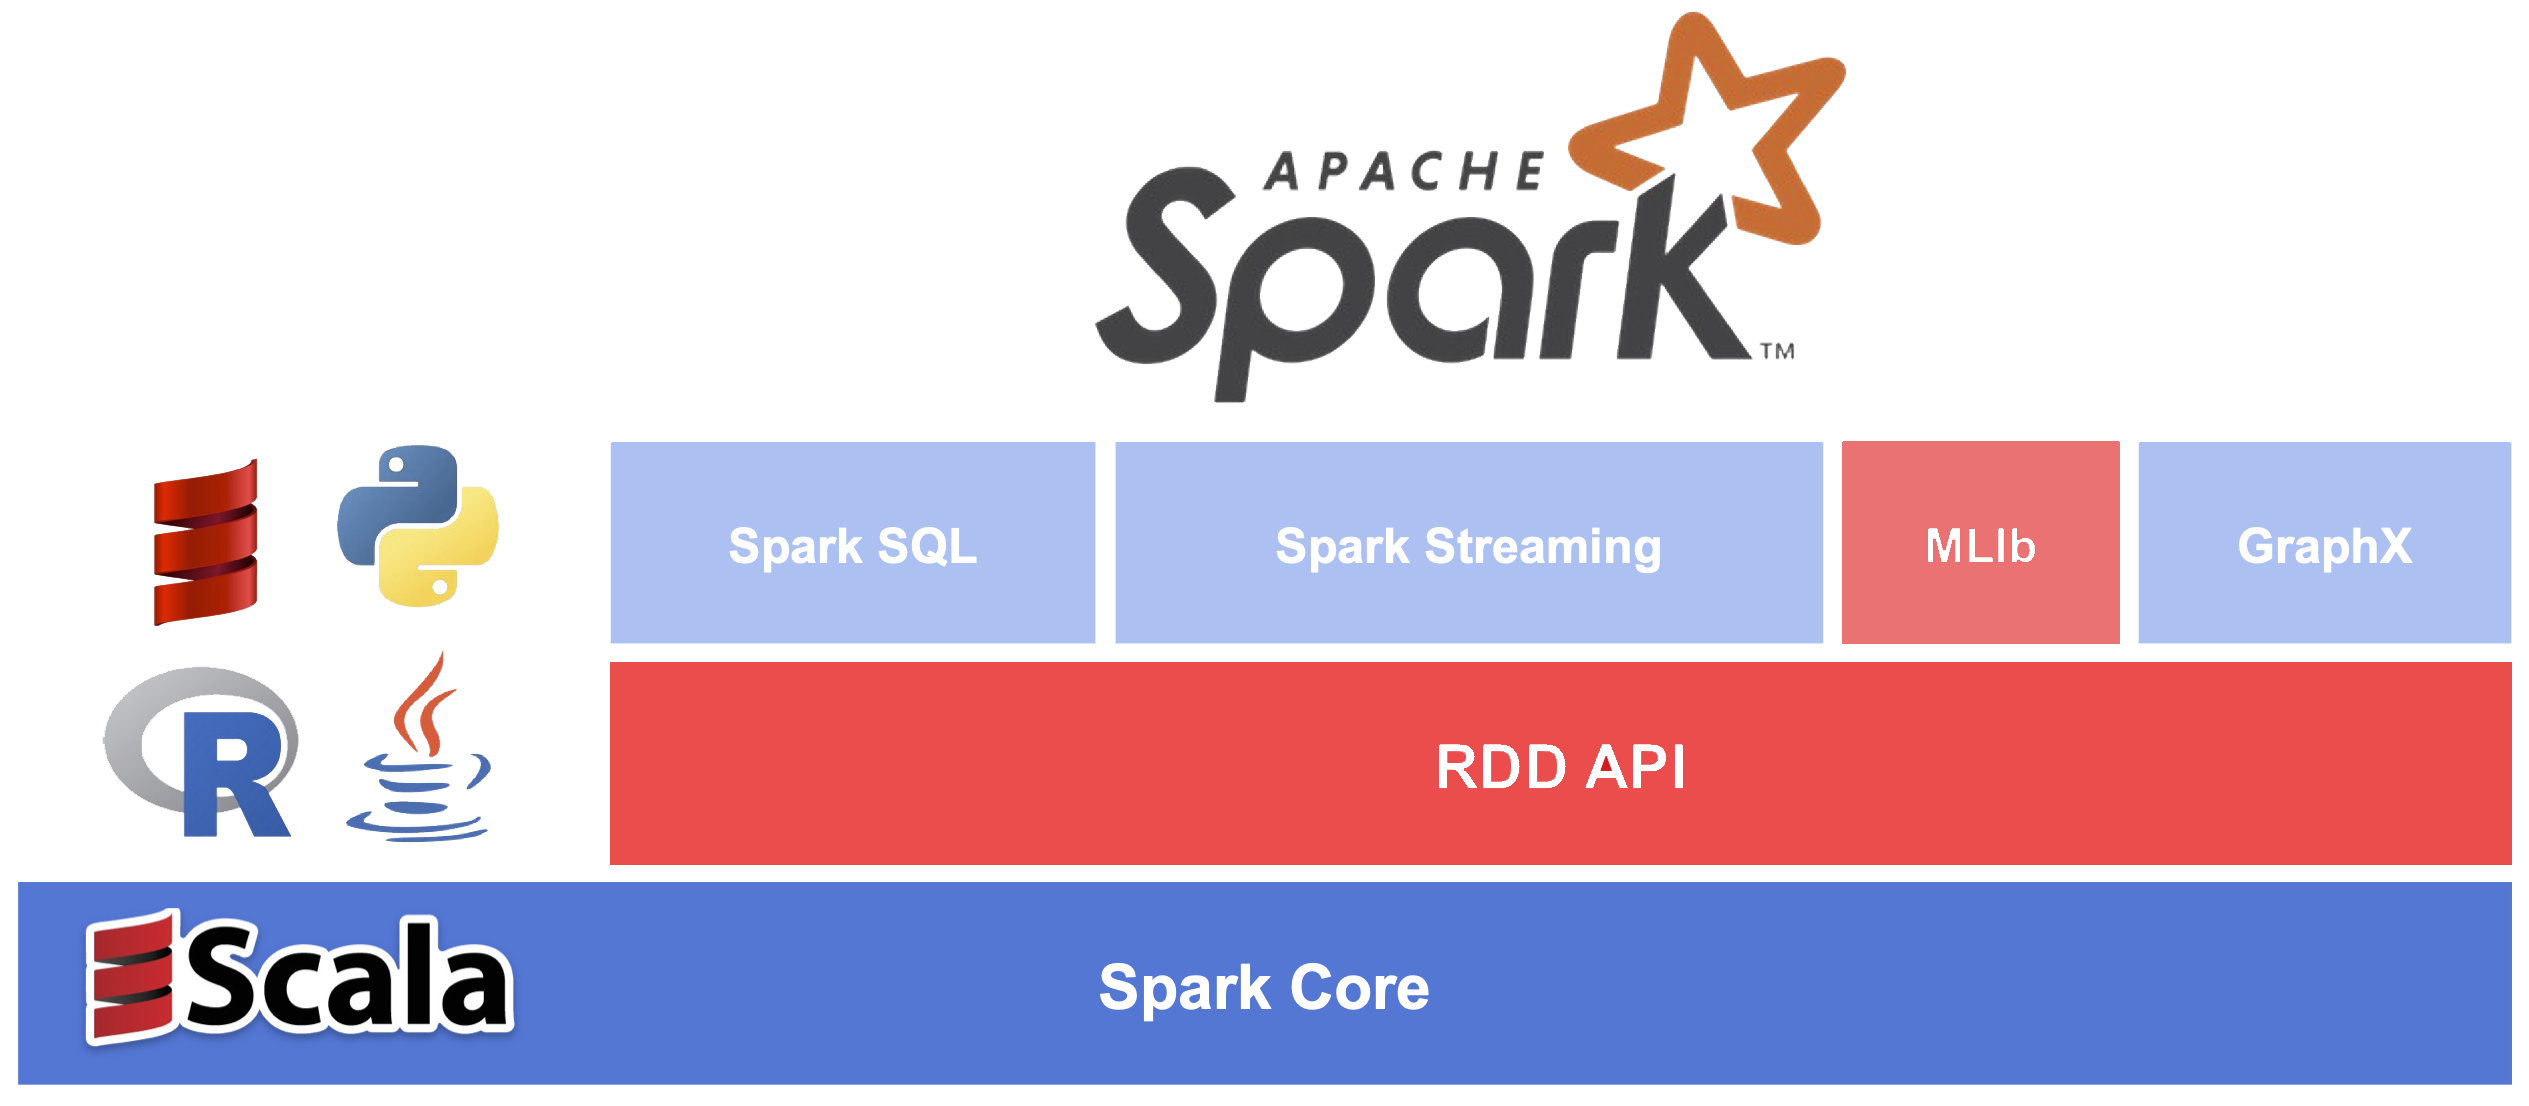
\includegraphics[width=0.9\textwidth]{figures/spark-overview-select.png}}
        \end{center}
        \end{block}
    \end{frame}

        \begin{frame}
            \frametitle{Spark}
            \framesubtitle{Architecture}
        \vspace{-4ex}
            \begin{block}{Spark Architecture}
            \begin{center}
                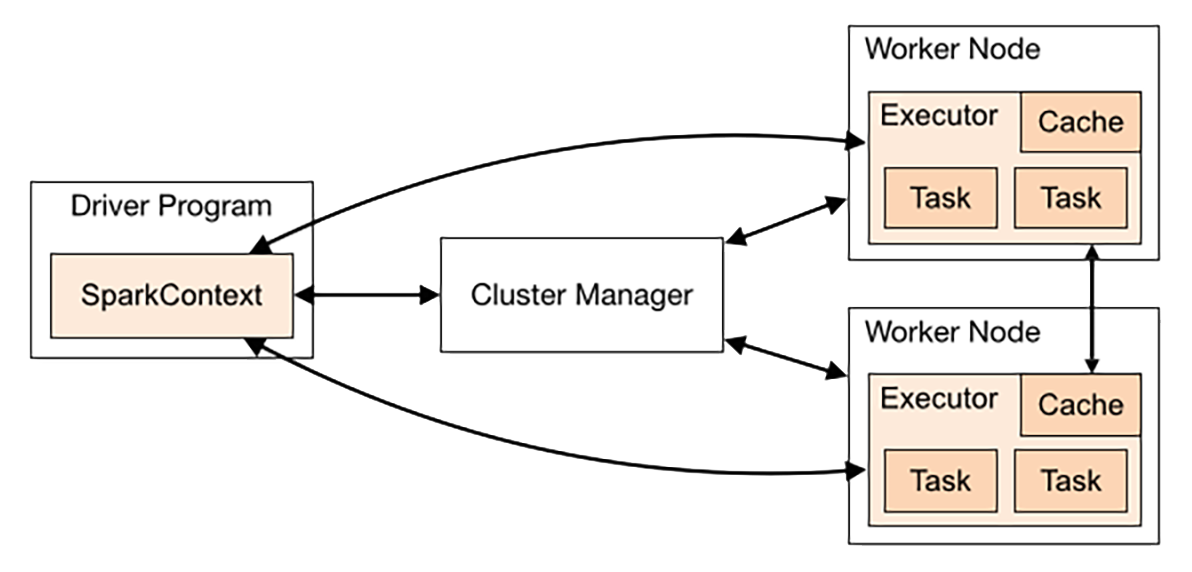
\includegraphics[width=0.9\textwidth]{spark-architecture.png}
            \end{center}
            \end{block}

        \end{frame}

        \begin{frame}
            \frametitle{Spark}
            \framesubtitle{RDD -- ``A read-only collection of records partitioned through the nodes in the cluster''}
            \begin{block}{RDD -- Resilient Distributed Dataset}
                When coding in Spark you work with RDDs. They are:
                \begin{itemize}
                    \item \alert{Immutable}
                    \item \alert{Distributed} and \alert{partitioned} in the cluster
                    \item \alert{Scalable} and \alert{fault tolerant}
                    \item Created from stored data or by transforming another RDD
                \end{itemize}
            \end{block}
        \end{frame}

        \begin{frame}
            \frametitle{Spark}
            \framesubtitle{RDD -- ``A read-only collection of records partitioned through the nodes in the cluster''}
            \begin{block}{Working with RDDs}
                \begin{itemize}
                    \item Spark can drop RDD's out of memory and they can then be \alert{recomputed at any time} as needed
                    \item We will be working with Python in this course, but
                    since Spark is written in Scala error messages will be \alert{Java
                    errors} and naming conventions are \alert{Java naming}. \alert{Don't worry about that!}
                \end{itemize}
            \end{block}
        \end{frame}

        \begin{frame}
            \frametitle{Spark}
            \framesubtitle{RDD -- ``A read-only collection of records partitioned through the nodes in the cluster''}
            \begin{block}{Transformations}
                A transformation 
                \begin{itemize}
                    \item creates a \alert{new RDD} from an old RDD
                    \item is evaluated \alert{lazily}
                \end{itemize}
            \end{block}
            \begin{block}{Actions}
                An action 
                \begin{itemize}
                    \item \alert{saves data} to file system or \alert{returns data} to driver program
                    \item \alert{blocks} while being evaluated
                \end{itemize}
            \end{block}
        \end{frame}

        \begin{frame}
            \frametitle{Spark}
            \framesubtitle{Dataframe}
            \begin{block}{Dataframe}
                When doing machine learning with Spark we will work a lot with
                dataframes. A dataframe consists of rows and columns.

                A bit like working with tables in Microsoft Excel \smiley{} 
            \end{block}
        \end{frame}

\subsection{Spark example}
        \begin{frame}
            \frametitle{Spark}
            \framesubtitle{Example}
            \begin{center}
                Now, let's look at some examples!
            \end{center}
        \end{frame}

    \begin{frame}[fragile]
        \frametitle{Example}
        \framesubtitle{Word counting (RDD)}
        \begin{center}

        \begin{minipage}{0.8\textwidth}
\begin{lstlisting}[escapechar={|}, title=wordcount.py]
|\only<1>{\color{black}}{\only<2->{\color{gray}}from pyspark.sql import SparkSession |

|\only<1>{\color{black}}{\only<2->{\color{Orchid}}spark = SparkSession.builder.appName("SimpleApp").getOrCreate()|
|\only<1>{\color{black}}{\only<2->{\color{Orchid}}sc = spark.sparkContext|

|\only<1>{\color{black}}{\only<2->{\color{NavyBlue}}rdd0 = sc.textFile("foo.txt")|

|\only<1>{\color{black}}{\only<2->{\color{NavyBlue}}rdd1 = rdd0.flatMap( lambda line : line.split(" ") ) \only<3>{\commentfont \color{darkpastelgreen} \# transformation}|
|\only<1>{\color{black}}{\only<2->{\color{NavyBlue}}rdd2 = rdd1.map( lambda word : (word,1) ) \only<3>{\commentfont \color{darkpastelgreen} \# transformation}| 
|\only<1>{\color{black}}{\only<2->{\color{NavyBlue}}rdd3 = rdd2.reduceByKey( lambda a,b : (a + b) ) \only<3>{\commentfont \color{darkpastelgreen} \# transformation}|

|\only<1>{\color{black}}{\only<2->{\color{BrickRed}}print(rdd3.collect()) \only<3>{\commentfont \color{darkpastelgreen} \# action}|
\end{lstlisting}
\end{minipage}
\end{center}
    \end{frame}

    \begin{frame}[plain]
    \hspace*{-1em}
            \begin{tikzpicture}[node distance= 25 pt]
        \only<1>{
        \node (txt)  [fill={rgb:purple,1;white,4}, draw,minimum height=.5cm,minimum width = .5cm, node distance = 55 pt]{foo bar foo bar buzz};
        \node [above of = txt, node distance = 14 pt] {\small\commentfont foo.txt };
        }

        \only<6>{
        \node (txt)  [fill={rgb:purple,1;white,4}, draw,minimum height=.5cm,minimum width = .5cm, node distance = 55 pt]{foo bar foo bar buzz};
        \node [above of = txt, node distance = 14 pt] {\small\commentfont foo.txt };
        }
        
        \uncover<2-5>{
        \node (txt)  [fill={rgb:purple,1;white,15}, draw,minimum height=.5cm,minimum width = .5cm, node distance = 55 pt]{foo bar foo bar buzz};
        \node [above of = txt, node distance = 14 pt] {\small\commentfont foo.txt };
        }
        
        \only<2->{
        \node (rdd0)  [fill={rgb:purple,1;white,4}, below of = txt, draw,minimum height=.5cm,minimum width = .5cm, node distance = 55 pt]{"foo bar foo bar buzz"};
        \node [above of = rdd0, node distance = 14 pt] {\small\commentfont rdd0 };
        \draw [->, shorten <=4pt, shorten >=4pt,out=-35, in=35] (txt) to node[right]
              {\color{NavyBlue}\small\texttt{rdd0 = sc.textFile("foo.txt")}} (rdd0);
        }

        \uncover<3->{
        \node (rdd0)  [fill={rgb:purple,1;white,15}, below of = txt, draw,minimum height=.5cm,minimum width = .5cm, node distance = 55 pt]{"foo bar foo bar buzz"};
        \node [above of = rdd0, node distance = 14 pt] {\small\commentfont rdd0 };
        \draw [->, shorten <=4pt, shorten >=4pt,out=-35, in=35] (txt) to node[right]
              {\color{NavyBlue!40!white}\small\texttt{rdd0 = sc.textFile("foo.txt")}} (rdd0);
        }
        
        \only<3->{
        \node (rdd1)  [fill={rgb:purple,1;white,4}, below of = rdd0, draw,minimum height=.5cm,minimum width = .5cm, node distance = 55 pt]{"foo", "bar", "foo", "bar", "buzz"};
        \node [above of = rdd1, node distance = 14 pt] {\small\commentfont rdd1 };
        \draw [->, shorten <=4pt, shorten >=4pt,out=-35, in=35] (rdd0) to node[right]
              {\color{NavyBlue}\small\texttt{rdd1 = rdd0.flatMap( lambda line : line.split(" ") )}} (rdd1);
        }

        \uncover<4->{
        \node (rdd1)  [fill={rgb:purple,1;white,15}, below of = rdd0, draw,minimum height=.5cm,minimum width = .5cm, node distance = 55 pt]{"foo", "bar", "foo", "bar", "buzz"};
        \node [above of = rdd1, node distance = 14 pt] {\small\commentfont rdd1 };
        \draw [->, shorten <=4pt, shorten >=4pt,out=-35, in=35] (rdd0) to node[right]
              {\color{NavyBlue!40!white}\small\texttt{rdd1 = rdd0.flatMap( lambda line : line.split(" ") )}} (rdd1);
        }
        
        \only<4->{
        \node (rdd2)  [fill={rgb:purple,1;white,4}, below of = rdd1, draw,minimum height=.5cm,minimum width = .5cm, node distance = 55 pt]
                      {("foo", 1), ("bar", 1), ("foo", 1), ("bar", 1), ("buzz", 1)};
        \node [above of = rdd2, node distance = 14 pt] {\small\commentfont rdd2 };
        \draw [->, shorten <=4pt, shorten >=4pt,out=-35, in=35] (rdd1) to node[right]
              {\color{NavyBlue}\small\texttt{rdd2 = rdd1.map( lambda word : (word,1) )}} (rdd2);
        }
        
        \uncover<5->{
        \node (rdd2)  [fill={rgb:purple,1;white,15}, below of = rdd1, draw,minimum height=.5cm,minimum width = .5cm, node distance = 55 pt]
                      {("foo", 1), ("bar", 1), ("foo", 1), ("bar", 1), ("buzz", 1)};
        \node [above of = rdd2, node distance = 14 pt] {\small\commentfont rdd2 };
        \draw [->, shorten <=4pt, shorten >=4pt,out=-35, in=35] (rdd1) to node[right]
              {\color{NavyBlue!40!white}\small\texttt{rdd2 = rdd1.map( lambda word : (word,1) )}} (rdd2);
        }
        
        \only<5->{
        \node (rdd3)  [fill={rgb:purple,1;white,4}, below of = rdd2, draw,minimum height=.5cm,minimum width = .5cm, node distance = 55 pt]
                      {("foo", 2), ("bar", 2), ("buzz", 1)};
        \node [above of = rdd3, node distance = 14 pt] {\small\commentfont rdd3 };
        \draw [->, shorten <=4pt, shorten >=4pt,out=-35, in=35] (rdd2) to node[right]
              {\color{NavyBlue}\small\texttt{rdd3 = rdd2.reduceByKey( lambda a,b : (a + b) )}} (rdd3);
        }
        
        \uncover<6->{
        \node (rdd3)  [fill={rgb:purple,1;white,4}, below of = rdd2, draw,minimum height=.5cm,minimum width = .5cm, node distance = 55 pt]
                      {("foo", 2), ("bar", 2), ("buzz", 1)};
        \node [above of = rdd3, node distance = 14 pt] {\small\commentfont rdd3 };
        \draw [->, shorten <=4pt, shorten >=4pt,out=-35, in=35] (rdd2) to node[right]
              {\color{NavyBlue!40!white}\small\texttt{rdd3 = rdd2.reduceByKey( lambda a,b : (a + b) )}} (rdd3);
         
        \draw [->, shorten <=4pt, shorten >=4pt,out=15, in=-15, line width=1mm, opacity=0.85, color={rgb:purple,1;white,1}] (rdd3) to node[right,text width=6cm]
              {\commentfont \Large Now we have made a word count of the original file} (txt);
        }
            \end{tikzpicture}
    \end{frame}

\begin{frame}[fragile]
        \frametitle{Example}
        \framesubtitle{Dataframe}
        \vspace*{-5ex}
        \begin{center}
        \begin{minipage}{0.8\textwidth}
\begin{lstlisting}[escapechar={|}, title=dataframe.py]
|\only<1>{\color{black}}{\only<2>{\color{gray}}from pyspark.sql import SparkSession |
|\only<1>{\color{black}}{\only<2>{\color{gray}}from pyspark.sql.functions import mean |

|\only<1>{\color{black}}{\only<2>{\color{Orchid}}spark = SparkSession.builder.appName("SimpleApp").getOrCreate()|

|\only<1>{\color{black}}{\only<2>{\color{NavyBlue}}df = spark.read.format("csv")\textbackslash |
         |\only<1>{\color{black}}{\only<2>{\color{NavyBlue}}.option("header", "true")\textbackslash |
         |\only<1>{\color{black}}{\only<2>{\color{NavyBlue}}.option("inferSchema", "true").load("bar.txt")|
|\only<1>{\color{black}}{\only<2>{\color{NavyBlue!50!white}}df.show()|

|\only<1>{\color{black}}{\only<2>{\color{NavyBlue}}res = df.select([mean('foo')])|
|\only<1>{\color{black}}{\only<2>{\color{NavyBlue!50!white}}res.show()|

|\only<1>{\color{black}}{\only<2>{\color{NavyBlue}}res = df.groupBy("id").mean("foo","bar")|
|\only<1>{\color{black}}{\only<2>{\color{NavyBlue!50!white}}res.show()|

\end{lstlisting}
\end{minipage}
\end{center}
        
\end{frame}
\newsavebox{\mydfshowlisting}
\newsavebox{\myresoneshowlisting}
\newsavebox{\myrestwoshowlisting}
\begin{lrbox}{\mydfshowlisting}
\begin{lstlisting}[basicstyle=\ttfamily\tiny, frame=none]
+---+---+---+
| id|foo|bar|
+---+---+---+
|  A|  3|  0|
|  B|  1|  1|
|  B|  0|  2|
+---+---+---+
\end{lstlisting}
\end{lrbox}

\begin{lrbox}{\myresoneshowlisting}
\begin{lstlisting}[basicstyle=\ttfamily\tiny, frame=none]
+------------------+
|          avg(foo)|
+------------------+
|1.3333333333333333|
+------------------+
\end{lstlisting}
\end{lrbox}

\begin{lrbox}{\myrestwoshowlisting}
\begin{lstlisting}[basicstyle=\ttfamily\tiny, frame=none]
+---+--------+--------+
| id|avg(foo)|avg(bar)|
+---+--------+--------+
|  B|     0.5|     1.5|
|  A|     3.0|     0.0|
+---+--------+--------+
\end{lstlisting}
\end{lrbox}

    \begin{frame}[plain]
    \hspace*{-1em}
            \resizebox{!}{1.15\textheight}{
            \begin{tikzpicture}[node distance= 25 pt]
            \small
        \only<1->{
        \node (txt)  [fill={rgb:purple,1;white,4}, draw,minimum height=.5cm, text width = 1.5cm, node distance = 55 pt]
{id,foo,bar
A,3,0
B,1,1
B,0,2};
        \node [above of = txt, node distance = 31 pt] {\footnotesize\commentfont bar.txt };
        }
        \uncover<2->{
        \node (txt)  [fill={rgb:purple,1;white,15}, draw,minimum height=.5cm, text width = 1.5cm, node distance = 55 pt]
{id,foo,bar
A,3,0
B,1,1
B,0,2};
        \node [above of = txt, node distance = 31 pt] {\footnotesize\commentfont bar.txt };
        }

        \only<2->{
        \node (load) [right of = txt, node distance = 7 cm, text width = 10cm]
              {\begin{minipage}{10cm}
\color{NavyBlue}\small\texttt
{ \begin{tabular}{r@{\hskip0pt}l}
df = spark&.read.format("csv")\textbackslash \\
          &.option("header", "true")\textbackslash \\
          &.option("inferSchema", "true").load("bar.txt") \\
   \end{tabular}}
              \end{minipage}
          };
        }
        \uncover<3->{
        \node (load) [right of = txt, node distance = 7 cm, text width = 10cm]
              {\begin{minipage}{10cm}
\color{NavyBlue!40!white}\small\texttt
{ \begin{tabular}{r@{\hskip0pt}l}
df = spark&.read.format("csv")\textbackslash \\
          &.option("header", "true")\textbackslash \\
          &.option("inferSchema", "true").load("bar.txt") \\
   \end{tabular}}
              \end{minipage}
          };
        }
        \only<3->{
        \node (select) [below of = load, node distance = 3.5cm] 
              {\color{NavyBlue}\small\texttt{ res1 = df.select([mean('foo')]) }};
        }
        \uncover<4->{
        \node (select) [below of = load, node distance = 3.5cm] 
              {\color{NavyBlue!40!white}\small\texttt{ res1 = df.select([mean('foo')]) }};
        }
  

        \only<2->{
        \draw [->, shorten <=4pt, shorten >=4pt,out=-35, in=35] (load) to node (dfshow) [fill=white]
              {\color{NavyBlue!40!white}\small\texttt{df.show()}} (select);

        \node (dfshowT)  [right of = dfshow, fill={rgb:purple,1;white,4}, draw,minimum height=.5cm, text width = 1.8cm, node distance = 65 pt]
        {\usebox\mydfshowlisting};
        \node [above of = dfshowT, node distance = 33 pt] {\footnotesize\commentfont df };
        }

        \uncover<3->{
        \draw [->, shorten <=4pt, shorten >=4pt,out=-35, in=35] (load) to node (dfshow) [fill=white]
              {\color{NavyBlue!20!white}\small\texttt{df.show()}} (select);

        \node (dfshowT)  [right of = dfshow, fill={rgb:purple,1;white,15}, draw,minimum height=.5cm, text width = 1.8cm, node distance = 65 pt]
        {\usebox\mydfshowlisting};
        \node [above of = dfshowT, node distance = 33 pt] {\footnotesize\commentfont df };
        }

        \uncover<4->{
        \node (groupby) [below of = select, node distance = 3cm] 
              {\color{NavyBlue}\small\texttt{ res2 = df.groupBy("id").mean("foo","bar") }};
        }
        \only<3->{
        \draw [->, shorten <=4pt, shorten >=4pt,out=-35, in=35] (select) to node (res1show) [fill=white]
              {\color{NavyBlue!40!white}\small\texttt{res1.show()}} (groupby);
        }
        \uncover<4->{
        \draw [->, shorten <=4pt, shorten >=4pt,out=-35, in=35] (select) to node (res1show) [fill=white]
              {\color{NavyBlue!20!white}\small\texttt{res1.show()}} (groupby);
        }
        \only<3->{
        \node (res1showT)  [right of = res1show, fill={rgb:purple,1;white,4}, draw,minimum height=.5cm, text width = 2.5cm, node distance = 75 pt]
        {\usebox\myresoneshowlisting};
        \node [above of = res1showT, node distance = 26 pt] {\footnotesize\commentfont res1 };
        }
        \uncover<4->{
        \node (res1showT)  [right of = res1show, fill={rgb:purple,1;white,15}, draw,minimum height=.5cm, text width = 2.5cm, node distance = 75 pt]
        {\usebox\myresoneshowlisting};
        \node [above of = res1showT, node distance = 26 pt] {\footnotesize\commentfont res1 };
        }

        \uncover<4->{
        \node (empty) [below of = groupby, node distance = 2.6cm]{};
        \draw [->, shorten <=4pt, shorten >=4pt,out=-35, in=35] (groupby) to node (res2show) [fill=white]
              {\color{NavyBlue!40!white}\small\texttt{res2.show()}} (empty);

        \node (res2showT)  [right of = res2show, fill={rgb:purple,1;white,4}, draw,minimum height=.5cm, text width = 2.8cm, node distance = 80 pt]
        {\usebox\myrestwoshowlisting};
        \node [above of = res2showT, node distance = 29 pt] {\footnotesize\commentfont res2 };
        }
            \end{tikzpicture}}
    \end{frame}

    \begin{frame}
        \frametitle{Example}
        \framesubtitle{Some commands}
        I will now give examples of some commands, these lists are in no way complete!
    \end{frame}

    \begin{frame}
        \frametitle{Example}
        \framesubtitle{Some commands}
        \oldBlock{RDD's}
            \begin{center}
            \begin{tabular}{ll}
            \toprule
            Command & Explanation \\
            \midrule
            \texttt{.take(n)} & Bring $n$ things from list to local Python environment \\
            \texttt{.collect()} & Bring all back to local, \alert{Don't do on big RDD's!} \\
            \texttt{.parallelize} & Put things on cluster from local \\
            \texttt{.count()} & Number of items in the list \\
            \texttt{.flatmap} & flatten structure ([[1,2],[3,4]] $\Rightarrow$ [1,2,3,4]) after applying a map \\
            \texttt{.reduceByKey} & merge values by key during reduce \\
            \bottomrule
            \end{tabular}
            \end{center}
        \endoldBlock
    \end{frame}
    
    \begin{frame}
        \frametitle{Example}
        \framesubtitle{Some commands}
        \oldBlock{Dataframes}
            \begin{center}
            \begin{tabular}{ll}
            \toprule
            Command & Explanation \\
            \midrule
            \texttt{.show()} & Print a representation of the dataframe \\
            \texttt{.printSchema()} & Print datatypes and other info about a dataframe \\
            \texttt{.coalesce} & Reduce number of partitions a dataset is spread over \\
            \bottomrule
            \end{tabular}
            \end{center}
        \endoldBlock
    \end{frame}

\section{QSAR}
\begin{frame}[plain]
\hfill\LARGE QSAR -- Quantitative structure–activity relationship \hfill\normalsize
\end{frame}

    \begin{frame}
        \frametitle{QSAR}
        \framesubtitle{Quantitative structure–activity relationship}

        \begin{block}{Quantitative structure–activity relationship}
            In QSAR we mathematically describe molecular structure and by machine learning predict molecular properties
            \uncover<2>{
            \begin{itemize}
                \item \alert{QSAR} -- Quantitative Structure-Activity Relationship
                \item \alert{QSPR} -- Quantitative Structure-Property Relationship
            \end{itemize}
            }
        \end{block}
    \end{frame}
    
    \begin{frame}
        \frametitle{QSAR}
        \framesubtitle{Quantitative structure–activity relationship}

        \begin{block}{Quantitative structure–activity relationship}
            QSAR can be used for predicting almost any molecular properties:
            \begin{itemize}
                \item Biological activity
                \item Risk management, toxicology
                \item \ldots
            \end{itemize}
        \end{block}

    \end{frame}

    \begin{frame}
        \frametitle{QSAR}
        \framesubtitle{Quantitative structure–activity relationship}
        \centering

        \begin{tikzpicture}
                \node (structures) [text width=2.4cm, rectangle, text centered]
                                  {Molecular structures};
                \node (activity) [text width=3cm, rectangle, 
                                text centered, right of=structures, node distance=3.5cm]
                                {Activity or Property};
                \only<1>{\draw [->] (structures) to (activity);}
                \uncover<2->{\draw [dashed,->] (structures) to (activity);}
            \uncover<2->{
                \node (descriptors) [text width=2.4cm,rectangle, node distance=1.5cm,
                                     text centered, below of=structures]
                                    {Molecular descriptors};
                \draw [->] (structures) to (descriptors);
            }
            \uncover<3->{
                \node (model) [text width=3cm,rectangle, node distance=1.5cm,
                                     text centered, below of=activity]
                                    {Mathematical model};
                \draw [->] (descriptors) to (model);
            }
            \uncover<4->{
                \draw [->] (model) to (activity);
            }
            \uncover<5->{
                \footnotesize
                \node (combine) [text width=3.5cm,rectangle, node distance=2.2cm,
                                     text centered, below left of=descriptors]
                                {\color{darkpastelgreen}Good to combine many different descriptors};
                \draw [->, darkpastelgreen] (combine) to (descriptors);
                \node (validation) [text width=5.6cm,rectangle, node distance=2.2cm,
                                     text centered, below right of=model]
                                {\color{darkpastelgreen}Machine learning};
                \draw [->, darkpastelgreen] (validation) to (model);
                \node (more) [text width=4cm,rectangle, node distance=2cm,
                                     text centered, above left of=structures]
                                {\color{darkpastelgreen}More structures often lead to better models};
                \draw [->, darkpastelgreen] (more) to (structures);
            }
        \end{tikzpicture}
    \end{frame}

    \subsection{Molecular Descriptors}
    \begin{frame}
        \frametitle{Molecular Descriptors}
                \begin{block}{Molecular descriptors} 
A molecular \alert{descriptor} is a \alert{mathematical representation} of a
molecule, often resulting from the \alert{transformation} of the \alert{symbolic
representation} of a molecule into \alert{numbers}
        \end{block}
    \uncover<2->{
    \begin{block}{Simple examples}
    \quad
    \begin{minipage}[c]{0.3\linewidth}
        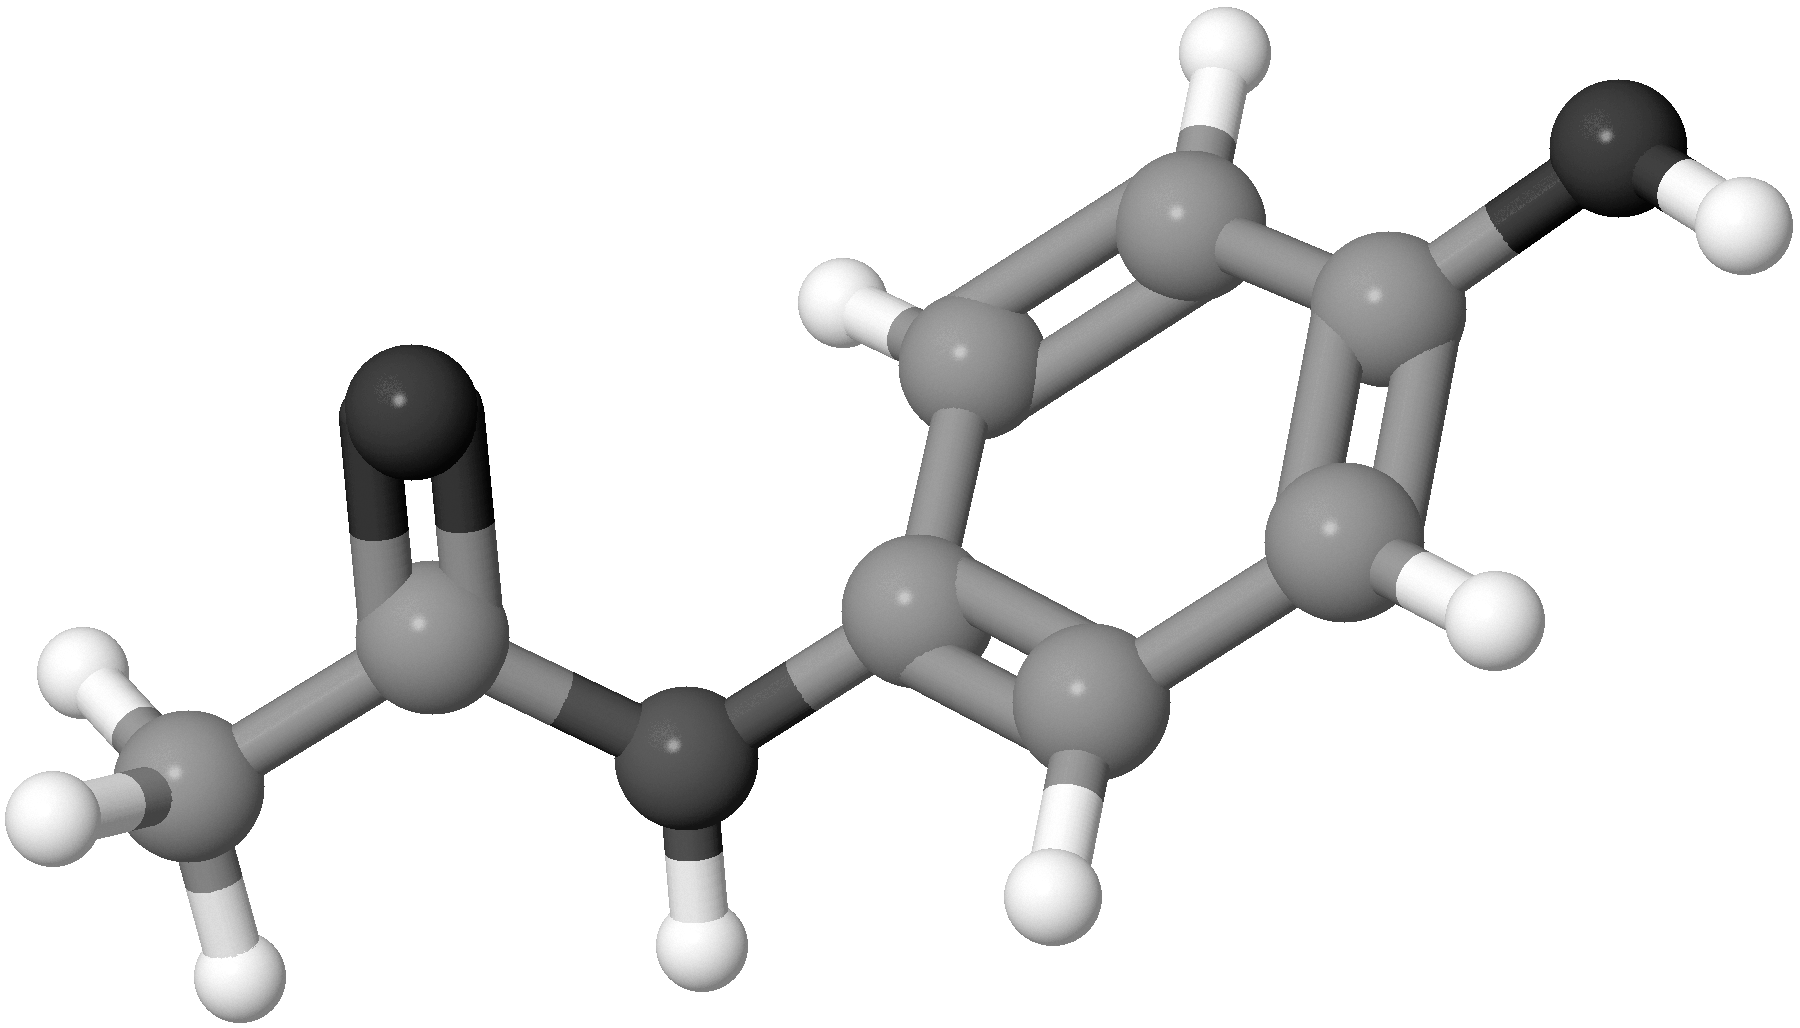
\includegraphics[width=1\textwidth]{figures/paracetamol.png}
    \end{minipage}
    \qquad
    \begin{minipage}[c]{0.4\linewidth}
    \small
    \begin{tabular}{lr}
    \toprule
    Descriptor & Value \\
    \midrule
    Molecular weight          & 151.06 \\
    Number of carbon atoms    & 8      \\
    \bottomrule
    \end{tabular}
    \end{minipage}
    \end{block}}

    \end{frame}

    \newcommand\tm[2][]{\tikz[overlay,remember picture,baseline=(#1.base),inner sep=0pt]\node(#1){$#2$};}

    \begin{frame}
        \frametitle{Molecular descriptors}
        \framesubtitle{Examples}
        \vspace{-4 ex}
        \begin{block}{Wiener index}
        \small
        The \alert{Wiener index} $W$ is defined as: the \alert{sum of the lengths} of the
        \alert{shortest paths between} all \alert{pairs of vertices} in the
        chemical graph of the molecule \alert{excluding hydrogens}. It can be
        calculated by \alert{summing the upper right triangle} of the
        \alert{distance matrix} $D$ for the compound:
        \small
        \begin{equation*}
            D\left( \raisebox{-2ex}{\chemfig{ C_a-C_b-[:50,,,1]O_cH }}\right)  = \begin{blockarray}{cccc}
        & \chemfig{C_a} & \chemfig{C_b} &  \chemfig{O_c} \\
            \begin{block}{c(ccc)}
        \chemfig{C_a} &  0 & \tm[a]{1} & \tm[b]{2} \\
        \chemfig{C_b} &  1 & 0 & \tm[c]{1}         \\
        \chemfig{O_c} &  2 & 1 & 0 \\
        \end{block}
        \end{blockarray},\qquad
        W = 1 + 2 + 1 = 4
        \end{equation*}
        \begin{tikzpicture}[overlay, remember picture]
        \node(x)[fit=(a) (b),inner sep=2pt]{};
        \node(y)[fit=(b) (c),inner sep=2pt]{};
        \fill[rounded corners,opacity=.3,fill=uured](x.north west)--(x.south west)--(y.south west)--(y.south east)--(x.north east)--cycle;
        \end{tikzpicture}
        \vspace{-1\baselineskip}
            \end{block}
    \end{frame}

    \begin{frame}
        \frametitle{Molecular Fingerprints}
        \begin{block}{Molecular Fingerprints}
            A molecular fingerprint is a \alert{list of numbers with a fixed length} that describes a molecule. Commonly they are \alert{bit fingerprints}:
            \begin{center}
          \begin{tikzpicture}[remember picture, node distance=0]
            \small
            \node (foo){};
            \node (a1)  [draw,minimum height=.5cm,minimum width = .5cm, below of = foo, node distance = 5 pt, xshift=.5cm, ]{$1$};
            \node (a2)  [draw,minimum height=.5cm,minimum width = .5cm, right of = a1, xshift=.5cm]{$0$};
            \node (a3)  [draw,minimum height=.5cm,minimum width = .5cm, right of = a1, xshift=1cm]{$1$};
            \node (a4)  [draw,minimum height=.5cm,minimum width = .5cm, right of = a1, xshift=1.5cm]{$0$};
            \node (a5)  [draw,minimum height=.5cm,minimum width = .5cm, right of = a1, xshift=2cm]{$1$};
            \node (a6)  [draw,minimum height=.5cm,minimum width = .5cm, right of = a1, xshift=2.5cm]{$0$};
            \node (a7)  [draw,minimum height=.5cm,minimum width = .5cm, right of = a1, xshift=3cm]{$0$};
            \node (a8)  [draw,minimum height=.5cm,minimum width = .5cm, right of = a1, xshift=3.5cm]{$1$};
          \end{tikzpicture}
          \end{center}

          but sometimes they are \alert{count fingerprints}:
          \begin{center}
          \begin{tikzpicture}[remember picture, node distance=0]
            \small
            \node (foo){};
            \node (a1)  [draw,minimum height=.5cm,minimum width = .5cm, below of = foo, node distance = 5 pt, xshift=.5cm, ]{$3$};
            \node (a2)  [draw,minimum height=.5cm,minimum width = .5cm, right of = a1, xshift=.5cm]{$0$};
            \node (a3)  [draw,minimum height=.5cm,minimum width = .5cm, right of = a1, xshift=1cm]{$5$};
            \node (a4)  [draw,minimum height=.5cm,minimum width = .5cm, right of = a1, xshift=1.5cm]{$0$};
            \node (a5)  [draw,minimum height=.5cm,minimum width = .5cm, right of = a1, xshift=2cm]{$1$};
            \node (a6)  [draw,minimum height=.5cm,minimum width = .5cm, right of = a1, xshift=2.5cm]{$0$};
            \node (a7)  [draw,minimum height=.5cm,minimum width = .5cm, right of = a1, xshift=3cm]{$0$};
            \node (a8)  [draw,minimum height=.5cm,minimum width = .5cm, right of = a1, xshift=3.5cm]{$9$};
          \end{tikzpicture}
          \end{center}
       \end{block}

    \end{frame}

        \begin{frame}
        \frametitle{Molecular descriptors}
        \framesubtitle{Molecular fingerprint / hashing}
        \begin{minipage}{0.95\textwidth}
        \oldBlock{Molecular fingerprint / hashing}
        \quad
            \begin{minipage}{0.45\textwidth}
                A \emph{simple} example of \alert{hashing} of a fingerprint using just
                \alert{position in alphabet}, \alert{summing up} the numbers for
                multi letter substances. 

                \vspace{0.5\baselineskip}
                Notice that we get a \alert{hash collision} for CL
                and O.  
            \end{minipage}
        \quad\tiny
            \begin{tabular}{cl}
                \toprule
                Molecules & Hash codes \\
                \midrule
                \chemfig[atom sep=2em]{HO-[:30]**6(---(-\Chemabove{N}{H}-[:-30](=[6]O)-[:30])---)}                          & 3, 14, 15 \\[2pt]  
                Atoms: C, N, O  &                                                                                         \\[14pt]
                \chemfig[atom sep=2em]{F-[:30](-[:90]F)-[:-30]O-[:30](-[:120]F)(-[:-60]F)-[:30](-[:90]F)-[:-30]Cl}          & 3, 6, 15  \\[4pt]
                Atoms: C, O, F, Cl                                                                            &           \\
                \bottomrule
            \end{tabular}
            \hspace{1em}
        \begin{minipage}{0.1\textwidth}
        \vfill
        \qquad
        \begin{tikzpicture}
            \tiny
            \node (box) [text width=1.7cm, rectangle, draw, text centered] { 
                $A=1$ \\ 
                $B=2$ \\ 
                $C=3$ \\
                \rotatebox[origin=c]{270}{$\ldots$} \\ 
                $F=6$ \\
                \rotatebox[origin=c]{270}{$\ldots$} \\ 
                $N=14$ \\ 
                $O=15$ \\ 
                \rotatebox[origin=c]{270}{$\ldots$} \\[1pt]
                $Cl=3+12$\\
                $=15$\\
                \rotatebox[origin=c]{270}{$\ldots$} \\ 
                };
        \end{tikzpicture}
        \vfill
        \end{minipage}
        \endoldBlock
        \end{minipage}
    \end{frame}

   \begin{frame}
        \frametitle{Molecular descriptors}
        \framesubtitle{Folding molecular fingerprints}

        \vspace{-6ex}
        \begin{minipage}{0.95\textwidth}
        \oldBlock{Molecular fingerprint -- folding}
        Imagine \alert{splitting} a fingerprint \alert{in half} and adding the
        two halves up using a \alert{logical~OR}. This is called
        \alert{folding}. 


    \begin{center}
    \hspace{-2.5cm}
    \begin{tikzpicture}[remember picture, node distance=0]
    \small
        \node (foo){};
        \node (a1)  [draw,minimum height=.5cm,minimum width = .5cm, below of = foo, node distance = 5 pt, xshift=.5cm, ]{$1$};
        \node (a2)  [draw,minimum height=.5cm,minimum width = .5cm, right of = a1, xshift=.5cm]{$0$};
        \node (a3)  [draw,minimum height=.5cm,minimum width = .5cm, right of = a1, xshift=1cm]{$1$};
        \node (a4)  [draw,minimum height=.5cm,minimum width = .5cm, right of = a1, xshift=1.5cm]{$0$};
        \node (a5)  [draw,minimum height=.5cm,minimum width = .5cm, right of = a1, xshift=2cm]{$1$};
        \node (a6)  [draw,minimum height=.5cm,minimum width = .5cm, right of = a1, xshift=2.5cm]{$0$};
        \node (a7)  [draw,minimum height=.5cm,minimum width = .5cm, right of = a1, xshift=3cm]{$0$};
        \node (a8)  [draw,minimum height=.5cm,minimum width = .5cm, right of = a1, xshift=3.5cm]{$1$};

        \node (arrow)  [minimum height=.5cm,minimum width = .5cm, right of = a1, xshift=4cm]{$\rightarrow$};
        \node (bar)  [minimum height=.5cm,minimum width = .5cm, right of = arrow, xshift=0.5cm]{};
        
        \node (b1)  [draw,minimum height=.5cm,minimum width = .5cm, above of = bar, node distance = 0.6 cm]{$1$};
        \node (b2)  [draw,minimum height=.5cm,minimum width = .5cm, right of = b1, xshift=0.5cm]{$0$};
        \node (b3)  [draw,minimum height=.5cm,minimum width = .5cm, right of = b1, xshift=1.0cm]{$1$};
        \node (b4)  [draw,minimum height=.5cm,minimum width = .5cm, right of = b1, xshift=1.5cm]{$0$};
        
        \node (or)  [minimum height=.5cm,minimum width = .5cm, right of = arrow, xshift=1.25cm]{OR};
        
        \node (c1)  [draw,minimum height=.5cm,minimum width = .5cm, below of = bar, node distance = 0.6 cm]{$1$};
        \node (c2)  [draw,minimum height=.5cm,minimum width = .5cm, right of = c1, xshift=0.5cm]{$0$};
        \node (c3)  [draw,minimum height=.5cm,minimum width = .5cm, right of = c1, xshift=1.0cm]{$0$};
        \node (c4)  [draw,minimum height=.5cm,minimum width = .5cm, right of = c1, xshift=1.5cm]{$1$};

        \node (arrow2)  [minimum height=.5cm,minimum width = .5cm, right of = or, xshift=1.25cm]{$\rightarrow$};
        
        \node (d1)  [draw,minimum height=.5cm,minimum width = .5cm, right of = arrow2, node distance = 0.5 cm]{$1$};
        \node (d2)  [draw,minimum height=.5cm,minimum width = .5cm, right of = d1, xshift=0.5cm]{$0$};
        \node (d3)  [draw,minimum height=.5cm,minimum width = .5cm, right of = d1, xshift=1.0cm]{$1$};
        \node (d4)  [draw,minimum height=.5cm,minimum width = .5cm, right of = d1, xshift=1.5cm]{$1$};

    \end{tikzpicture}
    \end{center}
        
    \uncover<2->{
    In fact a fingerprint can be folded into \alert{any
    final length}, making up a \alert{smaller and faster} to work with
    representation. Of course the shorter the fingerprint, the \alert{more
    features will correspond to each bit} and the \alert{more bits will be
    set to 1}.
    }
    

    \endoldBlock
    \end{minipage}

    \end{frame}

        \begin{frame}
        \frametitle{Molecular descriptors}
        \framesubtitle{The Morgan fingerprint}
        \centering
\resizebox{6em}{!}{
\chemfig[remember picturei, atom sep=1.5em]{
              NH_2% 7
    -[:270,,1]% 4
       -[:330]@{c1}% 3
                 (
            -[:30]% 8
                     (
                =[:90]O% 10
                     )
       -[:330,,,1]OH% 9
                 )
      =_[:270]% 2
       -[:210]% 1
      =_[:150]% 6
        -[:90]% 5
                 (
           =_[:30]% -> 4
                 )
}
\chemmove{
  \uncover<4->{\draw[-latex,shorten >=.4em, gray, thick, fill=uured, fill opacity=0.1]
    (a) node{} (c1.center) circle(2.7em);}
  \uncover<3->{\draw[-latex,shorten >=.4em, gray, thick, fill=uured, fill opacity=0.2]
    (b) node{} (c1.center) circle(1.8em);}
  \uncover<2->{\draw[-latex,shorten >=.4em, gray, thick, fill=uured, fill opacity=0.3]
    (a) node{} (c1.center) circle(0.8em);}
}
}

        \begin{block}{The Morgan fingerprint}
            Probably the most popular molecular fingerprint is the Morgan
            Fingerprint, also known as \alert{Extended Connectivity Fingerprint
            (ECFP)}. It is created by describing the neighbourhood of each atom
            out to a certain radius, \textit{i.e.}, distance from each atom, and
            then hashing (and sometimes folding) this down to a bit or count
            vector.
        \end{block}
    \end{frame}

\subsection{Similarity}

    \begin{frame}
        \frametitle{Using descriptors}
        \framesubtitle{Similarity}

        \begin{block}{Similarity}
            Having computed structural keys or descriptors we can use them for assessing the similarity of molecules.
            Perhaps you are familiar with distance measures such as:
            {\small
            \begin{equation*}
                \mbox{Euclidian distance}=\sqrt{\sum^n_{i=1}(q_i-p_j)^2} \quad 
                \mbox{Manhattan distance}=\sum_{i=1}^n{|p_i-q_i|}
            \end{equation*}}
        \end{block}
    \end{frame}


    \begin{frame}
        \frametitle{Using descriptors}
        \framesubtitle{Similarity}
        But most common in cheminformatics is probably:
        \begin{block}{Tanimoto similarity}
            {\small
            \begin{equation*}
            \mbox{Tanimoto similarity}=\frac{A \cap B}{ A \cup B}
                                    =\frac{\text{``Number of 1 in both keys''}}{\text{``Number of 1 in at least one key''}}
            \end{equation*}}
        \end{block}
     \end{frame}


    \begin{frame}
        \frametitle{Using descriptors}
        \framesubtitle{Similarity}
        \begin{block}{Example: Tanimoto similarity}
        \centering
            \begin{tabular}{rlr@{ }l}
            \toprule
            A:       & \texttt{10001001010101010100} \\
            B:       & \texttt{00011011010100101010} \\ [5pt]
            A and B: & \texttt{00001001010100000000} & 4&bits \\ [5pt]
            A or B:  & \texttt{10011011010101111110} & 13&bits \\
            \bottomrule
            \end{tabular}
            {\small\begin{equation*}
                \text{Tanimoto similarity}=\frac{\text{\scriptsize``Number of 1 in both keys''}}{\text{\scriptsize``Number of 1 in at least one key''}}=\frac{4}{13}\approx0.31
            \end{equation*}}
        \end{block}
    \end{frame}

    \subsection{The QSAR dataset}
        \begin{frame}  
            \frametitle{Using descriptors}
            \framesubtitle{The QSAR dataset}
                \begin{block}{A classification dataset}
                     \begin{center}
                     $\begin{NiceArray}{rccc}
                        & x_1 & x_2 & x_3 \\
                        \mathit{obs.~1} &  9 & 6 & 4 \\
                        \mathit{obs.~2} &  7 & 3 & 1 \\
                        \mathit{obs.~3} &  2 & 8 & 2 \\
                        \mathit{obs.~4} &  3 & 1 & 1 \\
                        \mathit{obs.~5} &  2 & 7 & 5 \\[12 pt]
                        \Block{1-4}{\textrm{X-matrix}} \\    
                     \CodeAfter
                        \SubMatrix[{2-2}{6-4}]
                    \end{NiceArray}$
                    \qquad
                     $\begin{NiceArray}{ccc}
                       & $y$   &\\
                       &     1 &\\
                       &     0 &\\
                       &     0 &\\
                       &     1 &\\
                       &     0 &\\[12 pt]
                        \Block{1-3}{\textrm{Y-column}} \\
                     \CodeAfter
                        \SubMatrix[{2-2}{6-2}]
                    \end{NiceArray}$
                \end{center}
                \end{block}
        \end{frame}

        \begin{frame}  
            \frametitle{Using descriptors}
            \framesubtitle{The QSAR dataset}
                \begin{block}{A regression dataset}
                     \begin{center}
                     $\begin{NiceArray}{rccc}
                        & x_1 & x_2 & x_3 \\
                        \mathit{obs.~1} &  9 & 6 & 4 \\
                        \mathit{obs.~2} &  7 & 3 & 1 \\
                        \mathit{obs.~3} &  2 & 8 & 2 \\
                        \mathit{obs.~4} &  3 & 1 & 1 \\
                        \mathit{obs.~5} &  2 & 7 & 5 \\[12 pt]
                        \Block{1-4}{\textrm{X-matrix}} \\    
                     \CodeAfter
                        \SubMatrix[{2-2}{6-4}]
                    \end{NiceArray}$
                    \qquad
                     $\begin{NiceArray}{ccc}
                       & $y$   &\\
                       &     0.123 &\\
                       &     0.320 &\\
                       &     0.590 &\\
                       &     1.000 &\\
                       &     0.095 &\\[12 pt]
                        \Block{1-3}{\textrm{Y-column}} \\
                     \CodeAfter
                        \SubMatrix[{2-2}{6-2}]
                    \end{NiceArray}$
                \end{center}
                \end{block}
        \end{frame}








    \setbeamertemplate{background}{%
        \parbox[c][\paperheight]{\paperwidth}{%
            \vskip -8 ex \hskip -2 em
            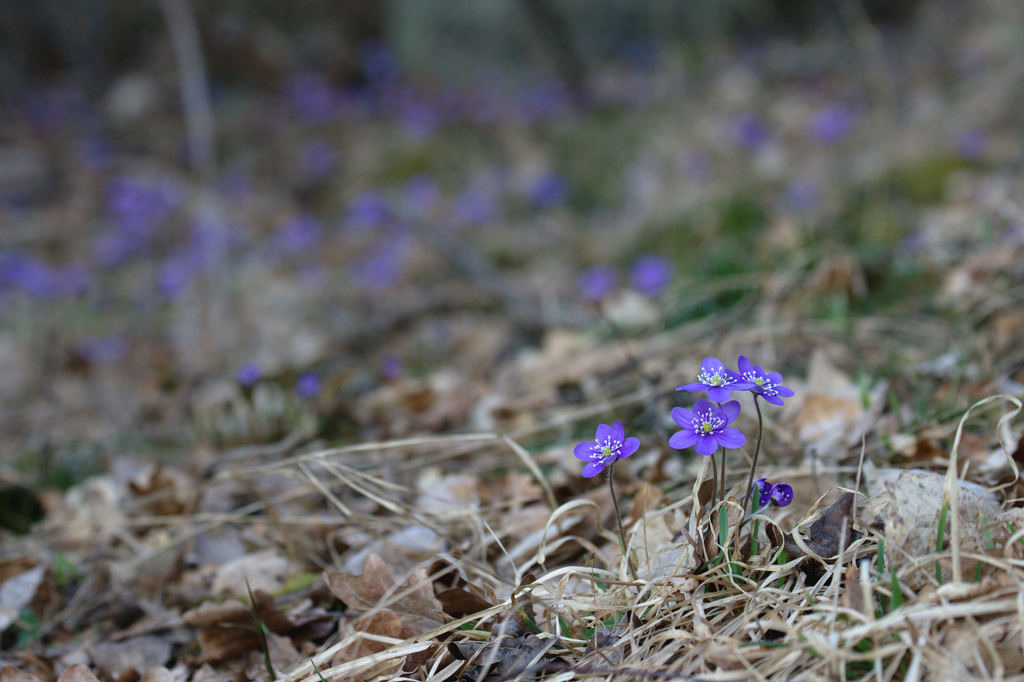
\includegraphics[height=1.5\paperheight]{Figures/blasippa.jpg}
        }   
        \parbox[c][\paperheight]{\paperwidth}{%
            \vskip 25 ex \hskip -40 em
            \color{white}\fbox{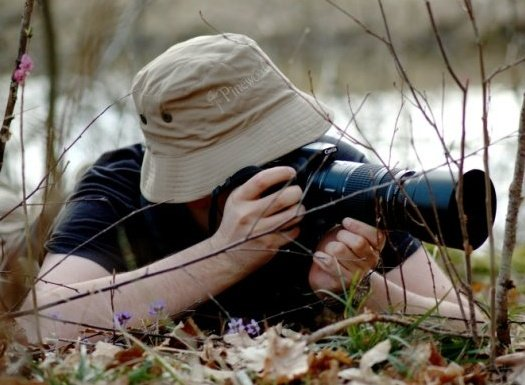
\includegraphics[height=0.37\paperheight]{Figures/me.jpg}}
        }   
    }
    \begin{frame}[plain]
        \vfill\hfill{\Huge\qquad\color{white} \zB Thank \zC you}\hfill\hfill\hfill\vfill
    \end{frame}
    \setbeamertemplate{background}{}

\end{document}
